%Kompiliuoti su XeLaTeX ir BibTeX

\documentclass[a4paper, 12pt, twoside]{article}

\usepackage[yyyymmdd]{datetime}

\usepackage{fontspec}
\usepackage{fontenc}
\usepackage{ulem}
\usepackage{cite}
\usepackage{mathtools}
\usepackage{amsmath}
\usepackage{amssymb}
%\usepackage{float}
\usepackage{graphicx}
\usepackage{multirow}
\usepackage[hyphens]{url}
\usepackage{caption}
\usepackage[svgnames]{xcolor}
\usepackage{lineno}
\usepackage[lithuanian]{babel}
\usepackage{hyperref}
\usepackage{siunitx}
\usepackage{floatrow}
\usepackage{indentfirst}
%\usepackage[parfill]{parskip}

\floatsetup[table]{capposition=top}

\hypersetup{breaklinks=true}
\urlstyle{same}

\usepackage{geometry}
\pagestyle{myheadings}
\geometry{
	left=2.5cm,
	right=2.5cm,
	top=3cm,
	bottom=3cm,
}
\pagenumbering{arabic}
\linespread{1.25}

\graphicspath{ {images/ataskaita/} }

\renewcommand{\dateseparator}{-}
\addto\captionslithuanian{\renewcommand{\figurename}{pav}}
\addto\captionslithuanian{\renewcommand{\refname}{5 \hspace{0.1cm} Naudotos literatūros sąrašas}}
\addto\captionslithuanian{\renewcommand{\tablename}{lentelė}}

\DeclareCaptionLabelFormat{numfirst}{#2~#1}
\captionsetup[figure]{labelformat = numfirst, labelsep = period}
\captionsetup[table]{labelformat = numfirst, labelsep = period}

\newcommand{\textblue}[1]{{\color{Blue}#1}}
\newcommand{\textred}[1]{{\color{Red}#1}}
\newcommand{\comment}[1]{\newline\textblue{#1}\newline}
\newcommand{\commentNL}[1]{\textblue{#1}\newline}
\newcommand{\commentMA}[1]{\textred{#1}\newline}
\newcommand{\ttt}[1]{\texttt{#1}}
\newcommand{\pT}{p_{\mathrm{T}}}
\newcommand{\ET}{E_{\mathrm{T}}}
\newcommand{\WW}{W\! W}
\newcommand{\ZZ}{Z\! Z}
\newcommand{\WZ}{W\! Z}
\newcommand{\tbarW}{\bar{t}W}
\newcommand{\ttbar}{t\bar{t}}
\newcommand{\emu}{e\mu}
\newcommand{\mumu}{\mu\mu}
\newcommand{\gJets}{\gamma\! +\!\mathrm{Jets}}
\newcommand{\WJets}{W\! +\!\mathrm{Jets}}
\newcommand{\dtW}{tW\! + \! \bar{t}W}
\newcommand{\DYee}{\mathrm{DY} \! \rightarrow \! ee}
\newcommand{\DYmumu}{\mathrm{DY} \! \rightarrow \! \mu\mu}
\newcommand{\DYtau}{\mathrm{DY} \! \rightarrow \! \tau\tau}
\newcommand{\DY}{\mathrm{DY}}
\newcommand{\ltq}[1]{{\quotedblbase{}#1\textquotedblleft{}}}
\newcommand{\Lumi}{{\cal L}_\mathrm{int}}
\newcommand{\invfb}{fb$^{-1}\,$}
\newcommand{\invpb}{pb$^{-1}\,$}
\newcommand{\QCD}{QC\! D}

\newlength\q
\setlength\q{\dimexpr .5\textwidth -2\tabcolsep}

\begin{document}
%\linenumbers

\begin{titlepage}
\centering
{\large Vilniaus universitetas \\ Fizikos fakultetas \\ Teorinės fizikos ir astronomijos institutas \par}
\vspace{3.5cm}
{\Large Marijus Ambrozas \par}
\vspace{0.3cm}
{\Large Drell-Yan proceso tyrimas analizuojant CERN CMS eksperimento 2016 metų protonų susidūrimų duomenis \par}
\vspace{0.8cm}
{\large Mokslinio darbo ataskaita \par}
\vspace{0.8cm}
%{\large Projekto nr. 09.3.3-LMT-K-712-10-0128 \par}
\vspace{3.5cm}
{\large \begin{tabular*}{0.9\textwidth}{@{\extracolsep{\fill}}ll}
Studentas & Marijus Ambrozas\tabularnewline[0.5cm]
Darbo vadovas & dr. Andrius Juodagalvis\tabularnewline[0.5cm]
\end{tabular*} \par}
\vspace{4cm}
{\large Vilnius $2019$\par}
\end{titlepage}


\clearpage
%\addtocounter{page}{1}
\addtocontents{toc}{\protect\setcounter{tocdepth}{2}}
\tableofcontents
\clearpage

\section{Įvadas}% \addcontentsline{toc}{section}{Įvadas}

Teoretikai protonų sandarą aprašo jų sudedamųjų dalių, vadinamų partonais, pasiskirstymo funkcijomis \cite{NNPDF}.
Norint geriau suprasti hadronų susidūrimuose vykstančius procesus, svarbu partonų pasiskirstymus žinoti kuo tiksliau.
Hadronų susidūrimų metu vykstančių reakcijų skerspjūviai yra apskaičiuojami kaip partonų pasiskirstymo
funkcijų ir partonų tarpusavio reakcijos skerspjūvio kombinacija.
Kvantinės chromodinamikos teorija nenumato tikslių partonų pasiskirstymo funkcijų išraiškų, todėl jas bandoma
apskaičiuoti pasinaudojant įvairių procesų eksperimentinių tyrimų rezultatais \cite{NNPDF, PDF_CTEQ, PDF_ABMP16}.

Drell-Yan procesas \cite{DYoriginal} -- tai toks procesas, kai protonų susidūrimo metu kvarkas iš vieno protono ir antikvarkas
iš kito anihiliuoja sukurdami virtualų fotoną arba $Z$ bozoną, kuris netrukus skyla į leptono ir antileptono porą.
Skirtingos Drell-Yan proceso galutinės būsenos, priklausomai nuo to, kokios rūšies leptonai susidaro, yra
vadinamos kanalais: elektronų kanalas, miuonų kanalas, taonų kanalas.
%Drell-Yan proceso aprašymas, naudojantis perturbacine kvantine chromodinamika, yra gerai išplėtotas iki antros
%eilės perturbacijų tikslumo (angl.\ \textit{next-to-next-to-leading order} -- NNLO) \cite{DYNNLO, DYrapiNNLO, VecBosonNNLO}.
Ypatingai tiksliai atliekamų naujausių Drell-Yan proceso diferencialinio reakcijos skerspjūvio eksperimentinių matavimų
rezultatai \cite{DY2015, DY2018} pasitarnauja partonų pasiskirstymo funkcijų tikslinimui, perturbacinės kvantinės chromodinamikos bei
elektrosilpnosios sąveikos teorijų tikrinimui, taip pat ir kituose eksperimentiniuose didelių energijų fizikos
tyrimuose, kur Drell-Yan procesas yra dominuojantis triukšmas \cite{Higgs2018, Zprime, SUSYtau}.
Taigi, tikslūs Drell-Yan proceso matavimai yra visokeriopai svarbūs dalelių fizikos mokslui.

CERN Didysis hadronų greitintuvas vykdo labai galingus $13$ TeV energijos protonų susidūrimus \cite{DY2018}.
Egzistuoja tikimybė, kad tokių susidūrimų metu bus sukurtos nestabilios didelės masės dalelės,
kurių vidutinė gyvavimo trukmė yra labai trumpa.
Aplink protonų susidūrimo vietas išdėstytais dalelių detektoriais įmanoma užregistruoti tik tokių
dalelių skilimo produktus: fotonus, elektronus, įvairius hadronus bei miuonus.
Drell-Yan proceso tyrime ieškoma įvykių, kurių metu susidarė leptono-antileptono pora.
Egzistuoja ir taip vadinami triukšmo įvykiai, kurių galutinis produktas atrodo labai panašiai
į galutinį Drell-Yan proceso produktą.
Kadangi paėmus vieną konkretų užregistruotą įvykį neįmanoma atskirti, ar jis yra signalo
(Drell-Yan), ar triukšmo įvykis, į triukšmų indėlį reikia atsižvelgti statistiškai įvertinant,
kokią dalį tarp visų atrinktų įvykių jie galėjo sudaryti.

Šiame darbe buvo atliekama panašių į Drell-Yan įvykių atranka bei triukšmo įvykių skaičiaus įvertinimas $\emu$ metodu.
Darbas buvo atliktas naudojant CERN CMS eksperimento 2016 metais užregistruotus protonų susidūrimų duomenis.

\section{Metodika}
\subsection{Didysis hadronų greitintuvas ir Kompaktiškasis miuonų solenoidas}

Europos branduolinių tyrimų organizacijai CERN priklausantis Didysis hadronų greitintuvas
(angl.\ \textit{Large Hadron Collider} -- LHC) yra didžiausias ir galingiausias dalelių greitintuvas pasaulyje.
Maždaug $27$ km perimetro žiedinis greitintuvas slepiasi apytiksliai $100$ m gylyje po žeme \cite{LHC}.
Nuo $2015$ metų Didžiajame hadronų greitintuve vykstančių protonų susidūrimų energija sieka net $13$ TeV.
Įprastai jie vyksta kas $25$ ns keliuose skirtinguose žiedo taškuose, aplink kuriuos yra išdėstyti dalelių
detektoriai, priklausantys skirtingų eksperimentų grupėms.

Kompaktiškasis miuonų solenoidas (angl.\ \textit{Compact Muon Solenoid} -- CMS) yra plačios paskirties
detektorius, sukurtas skirtingų dalelių detektavimui.
CMS yra cilindrinės geometrijos, jo aukštis ir plotis -- apytiksliai po $15$ m, o ilgis --
apie $21$ m.
Detektoriaus masė siekia apie $14000$ tonų.
Detektorius susideda iš daug sluoksnių ir segmentų, kurie skirti detektuoti skirtingų rūšių dalelėms.
CMS \ltq{širdis} -- didžiausias pasaulyje solenoidinis elektromagnetas.
Tai -- iki superlaidumo temperatūros atšaldoma ritė, kuria darbo metu teka maždaug $19.1$ kA stiprio
elektros srovė, ir kurios viduje sukuriamas iki $4$ T siekiantis magnetinis laukas.

\vspace{0.2cm}
\begin{figure}[H]
	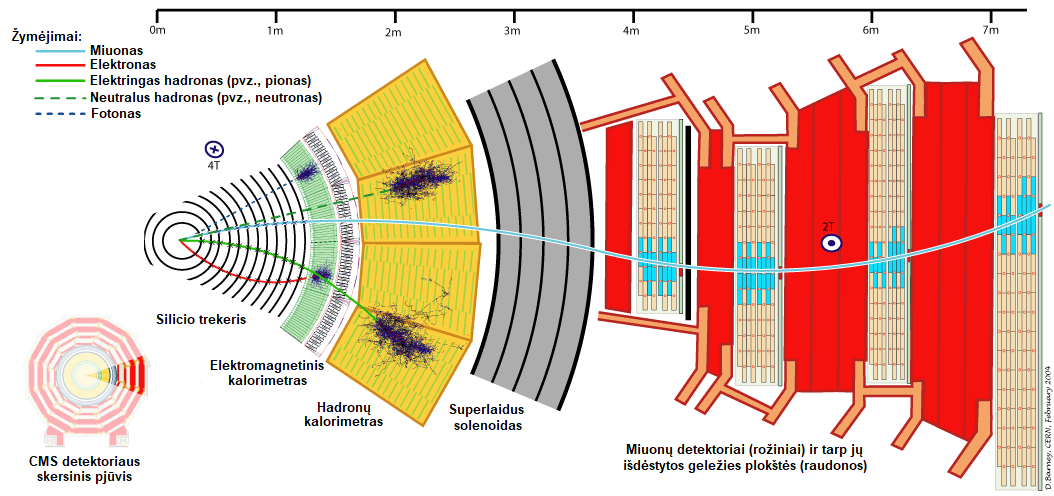
\includegraphics[width=\textwidth]{CMSslice_LT.png}
	\caption{\label{fig:CMSslice}Skersinis CMS detektoriaus pjūvis \cite{CMSslice}.
	Skirtingos linijos žymi skirtingų dalelių, išlekiančių iš protonų susidūrimo vietos, trajektorijas.
	Trūki linija žymi elektriškai neutralios dalelės trajektoriją, kuri silicio trekų detektoriuje
	neužfiksuojama.}
\end{figure}

CMS detektoriaus sluoksnius galima pamatyti \ref{fig:CMSslice} paveiksle.
Kiekvienas subdetektorius turi vieną cilindrinę ir dvi antgalių dalis, kurios yra sluoksniškai išdėstytos
aplink protonų susidūrimo vietą.
Kiekvienas subdetektorių sluosknis yra skirtingas ir turi savo paskirtį \cite{CMSexperiment}.

Kadangi detektoriaus elektronika nėra pajėgi išsaugoti kiekvieną kas $25$ ns vykstantį įvykį, išsaugomų
įvykių skaičiui sumažinti naudojama dviejų lygių trigerių sistema \cite{CMStrig}.
Pirmojo lygio trigeris -- tai šalia detektoriaus sumontuota specialiai tam sukurta kompiuterinės
įrangos sistema.
Joje realiu laiku minimaliai apdorojami kalorimetrų bei miuonų detektorių duomenys ir pagal juos per
$4 \; \mathrm{\mu s}$ sistema nusprendžia, ar įvykis turėtų būti išsaugomas tolimesnei analizei. 
Pirmojo lygio trigeris išsaugo tik maždaug $1$ įvykį iš $10000$.
Aukšto lygio trigeris -- tai superkompiuterių sistema, į kurią atkeliauja pirmojo lygio trigerį
aktyvavę įvykiai.
Čia įvykiai atkuriami pasinaudojant pilna detektoriaus užregistruota informacija, bei naudojami
griežtesni atrankos kriterijai.
Tai padeda įvykių skaičių sumažinti iki maždaug $1000$ įvykių per sekundę, kurie įrašomi ilgalaikiam saugojimui,
kad vėliau galėtų būti tyrinėjami mokslininkų.

Protonų susidūrimo įvykio vaizdas, pasinaudojant detektoriaus užregistruota informacija, atkuriamas naudojantis
dalelių srauto (angl. \textit{Particle Flow}) algoritmu \cite{ParticleFlow}.
Šis algoritmas bando susieti trekų detektoriuje užregistruotus signalus su pataikymais į kalorimetrus arba miuonų
detektorius, taip nustatydamas, kokios dalelės susidarė bei kokie jų parametrai (krūvis, skersinis impulsas,
skersinė energija, pseudosparta ir pan.).
Tokiu būdu gaunamas platus įvykio galutinių produktų sąrašas, leidžiantis pamatyti pilną įvykio vaizdą.

\subsection{Signalas ir triukšmas}

Drell-Yan proceso metu susidaro du priešingo krūvio leptonai.
Tokia pora gali susidaryti ir kitų procesų metu.
Tai -- \ltq{triukšmo įvykiai}.
Pagrindiniai Drell-Yan proceso triukšmai yra šie: viršūninių kvarkų poros ($t\bar{t}\,$) įvykiai, dviejų bozonų
įvykiai ($WW$, $WZ$ ir $ZZ$), vieno viršūninio kvarko ir $W$ bozono įvykiai ($tW$ arba $\bar{t}W$), $W$ bozono
ir čiurkšlės įvykiai ($\WJets$) bei stipriosios sąveikos nulemti kelių čiurkšlių įvykiai (sutrumpintai vadinami $\QCD$).
Taip pat tiriant Drell-Yan proceso elektronų ir miuonų kanalus vienas iš svarbių triukšmų yra
to paties Drell-Yan proceso taonų kanalas $\DYtau$, kai taonai skyla į elektronus arba miuonus.
Stengiantis išskirti, kokią dalį detektoriaus registruojamuose pasiskirstymuose sudaro signalo (Drell-Yan),
o kokią -- triukšmo įvykiai, yra pasitelkiamas Monte Carlo (MC) modeliavimas ir/arba matavimu grįsti metodai.

Monte Carlo modeliavimas -- tai Monte Carlo metodu sumodeliuoti protonų susidūrimo įvykiai.
Įvykių modeliavimas atliekamas keliais lygmenimis.
Pirmiausia sumodeliuojamas pats protonų susidūrimas ir gaunama, kokios dalelės susidarė jo metu.
Tada modeliuojami po susidūrimo vykstantys antriniai procesai, tokie, kaip hadronizacija, spinduliavimas ir dalelių skilimai.
Galiausiai modeliuojama detektoriaus sąveika su visais įvykio produktais.
Tokį virtualų eksperimentą kartojant daug kartų galima gauti vidutinį rezultatą, kuris yra palyginamas su eksperimentu.
Vis dėlto, sumodeliuoti įvykius taip, kad virtualaus eksperimento sąlygos idealiai atitiktų realaus eksperimento sąlygas,
yra praktiškai neįmanoma.
Norint atsižvelgti į kai kuriuos iš neatitikimų modeliuotiems įvykiams galima pritaikyti tam tikras pataisas.
Tačiau vis tiek egzistuoja neapibrėžtumų, tokių, kaip nepakankamos žinios apie atskirų triukšmo procesų įvykių tikėtinumus,
neidealus detektoriaus atsako modeliavimas, papildomi protonų susidūrimai ir pan., kurie kenkia įverčio kokybei.
Šių problemų gali būti išvengiama triukšmo įvykių skaičiaus įvertinimui naudojant matavimu grįstus metodus.

Matavimu grįsti metodai apjungia matavimą ir modeliavimą, kad būtų gautas kuo tikroviškesnis įvykių skaičiaus įvertis.
Pagrindinis matavimu grįstų įvykių skaičiaus įvertinimo metodų principas remiasi signalo ir kontrolinės sričių apibrėžimais.
Signalo sritis -- tai sritis, pasirinkta taip, kad į ją patektų kuo daugiau signalo ir kuo mažiau triukšmo įvykių.
Kontrolinė sritis -- tai taip pasirinkta sritis, kad į ją patektų kuo daugiau triukšmo ir kuo mažiau signalo įvykių.
Šios dvi sritys turi būti nepersiklojančios.
Skirtingi matavimu grįsti metodai įvairiais būdais transformuoja triukšmo įvykių skaičių, apskaičiuotą kontrolinėje
srityje, į triukšmo įvykių skaičių, patenkantį į signalo sritį.
Eksperimentinėje didelių energijų fizikoje ganėtinai populiarūs yra klaidingo fizikinio objekto atpažinimo ir ABCD metodai.
Jie naudojami įvertinti skaičiui tokių triukšmo įvykių, kurių metu susidarė čiurkšlės.
Triukšmų, siejamų su procesais, kurių metu susidariusios dvi nestabilios dalelės skyla į leptonus nepriklausomai ir su
vienodomis tikimybėmis, indėliui įvertinti naudojamas $\emu$ metodas, kuris ir buvo taikomas šiame darbe.

\subsection{Duomenų rinkiniai}

Šiame darbe buvo naudojami dalinai apdoroti CERN CMS detektoriaus 2016 metais užregistruoti $13$ TeV
energijos protonų susidūrimų duomenys, atitinkantys $35.9$ \invfb inte-gruotąjį šviesį, arba maždaug
$2 \cdot 10^{15}$ protonų susidūrimų.
Tai yra virš $10$ kartų daugiau įvykių, nei užregistruota $2015$-aisiais metais \cite{DY2018}.

Taip pat darbe buvo naudojami modeliuoto Drell-Yan signalo ir pagrindinių triukšmo procesų duomenų rinkiniai.
Drell-Yan signalo bei $\WJets$ proceso duomenų rinkiniai buvo sumodeliuoti naudojant
\textsc{MadGraph5\_aMC@NLO} įvykių modeliavimo programą \cite{MG_aMCatNLO}.
Viršūninio-antiviršūninio kvarko poros ($t\bar{t}\,$) ir vieno viršūninio kvarko kartu su $W$ bozonu ($tW$ arba
$\bar{t}W$) įvykiai buvo sumodeliuoti naudojant \textsc{Powheg} \cite{powheg_ttbar, powheg_tW}.
Visi šie išvardinti procesai buvo sumodeliuoti pirmos eilės perturbacijų tikslumu (angl.
\textit{next-to-leading order} -- NLO).
Dviejų bozonų ($WW$, $WZ$, $ZZ$) įvykiai buvo sumodeliuoti su \textsc{Pythia8} nulinės eilės perturbacijų tikslumu
(angl. \textit{leading order} -- LO) \cite{pythia82}.
Detektoriaus atsakas į kiekvieną iš sumodeliuotų įvykių buvo modeliuojamas naudojantis \textsc{Geant4} programa
\cite{geant4}.

Visi naudoti duomenys saugomi Pietų Korėjos Tier3 duomenų centre ir užima apie $14$ TB.
Duomenų išdėstymo struktūra schematiškai pavaizduota \ref{fig:duomSchem} pav.
Saugomi duomenys yra skirstomi į modeliuotus ir užregistruotus CMS detektoriumi.
CMS detektoriumi užregistruoti duomenys yra skirstomi į pirminius duomenų rinkinius pagal pirmo lygio trigerio
suveikimą, o pirminiai duomenų rinkiniai dar smulkiau skirstomi pagal duomenų registravimo laikotarpį.
Modeliuoti duomenys yra skirstomi pagal tai, kokio proceso įvykiai yra sumodeliuoti ir, kai kuriais atvejais,
dar yra smulkinami pagal tam tikrus įvykių parametrus (pavyzdžiui, įvykio metu sukurtos dalelės invariantinę masę,
skersinį impulsą ir pan.).
Kai kurie modeliuoti duomenų rinkiniai turi po keletą versijų arba plėtinių.
Duomenų analizei buvo rašomi C++ programiniai moduliai.
Duomenų rinkinių valdymui skirto programinio kodo struktūra buvo sukurta taip, kad jos loginių elementų išdėstymas
būtų panašus į duomenų struktūrą -- kintamasis \ttt{Process\_t} žymi modeliuotus procesus arba pirminius
eksperimentinių duomenų rinkinius, o adresų vektorius laiko skirtingų modeliuotų duomenų versijų arba skirtingų
duomenų registravimo laikotarpių pirminių duomenų rinkinių adresus.
Pagrindinių kodo elementų sąsajos su duomenų išdėstymu schematiškai pavaizduotos \ref{fig:duomKod} pav.

\begin{figure}[H]
	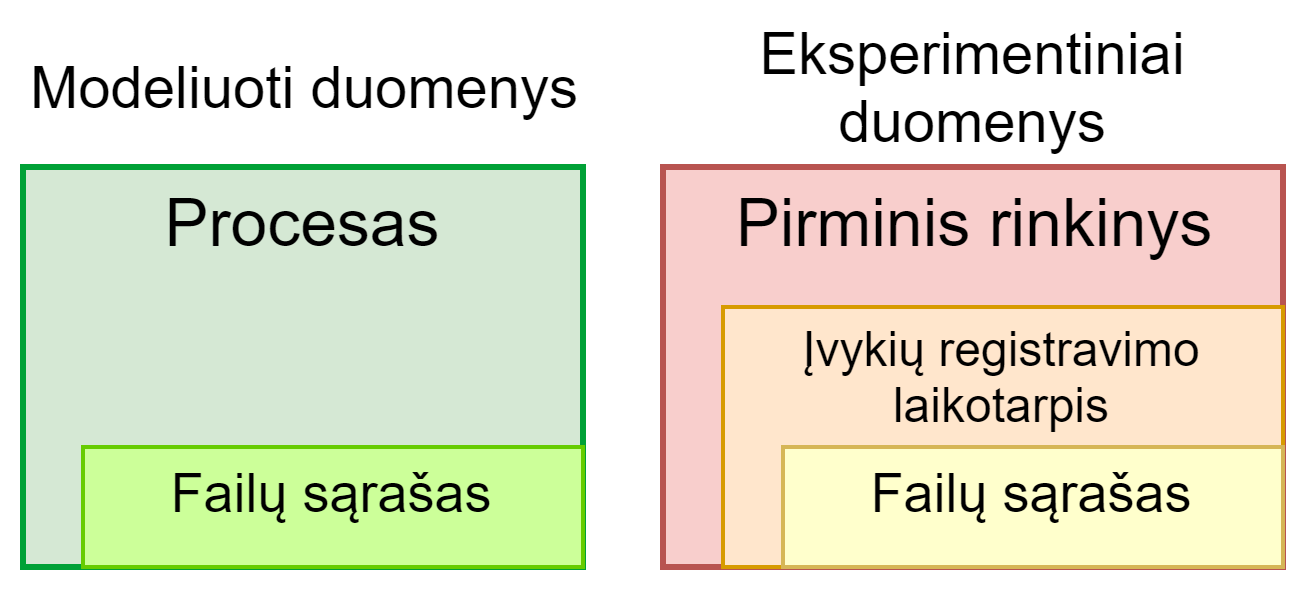
\includegraphics[width=\textwidth]{Duomenu_schema_DataMC_v2.png}
	\caption{\label{fig:duomSchem} Duomenų saugojimo schema.}
\end{figure}

\begin{figure}[H]
	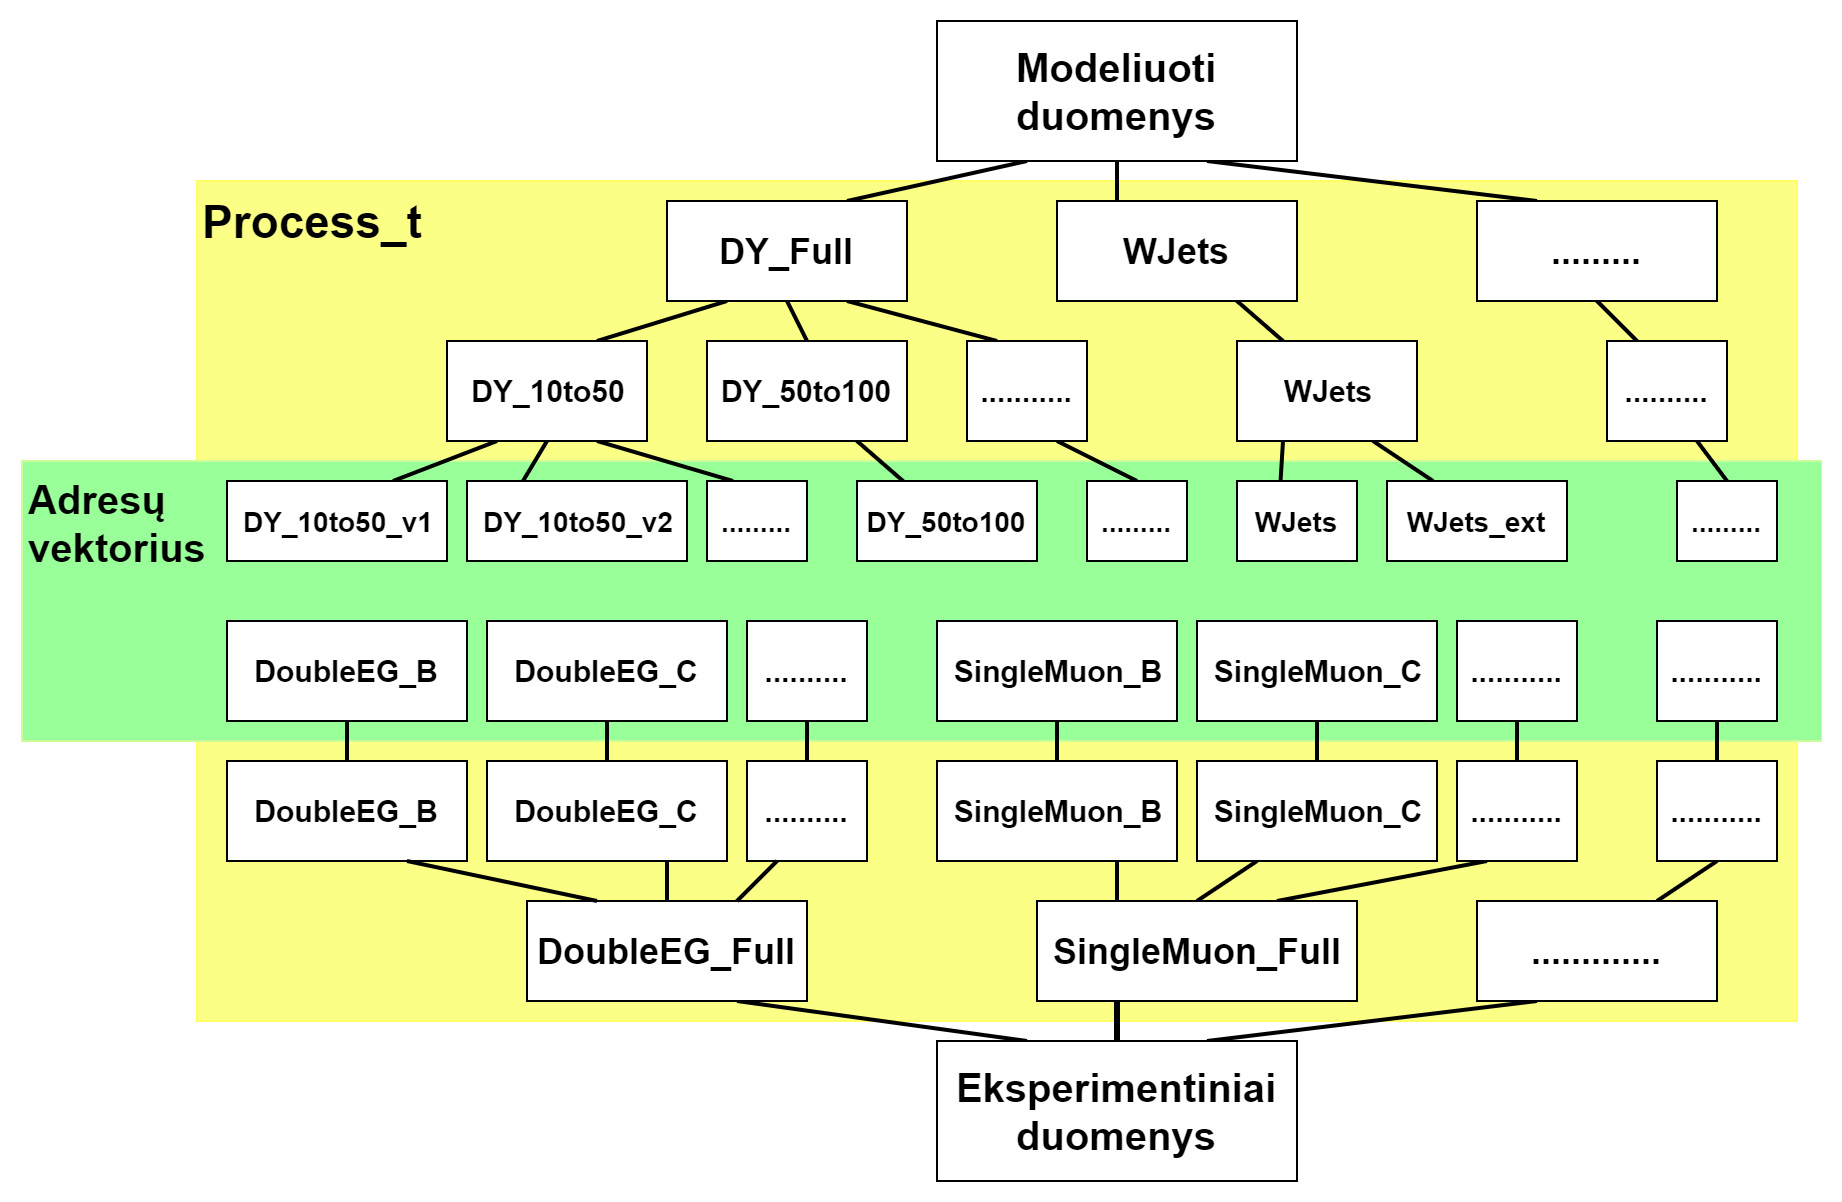
\includegraphics[width=\textwidth]{medis_praplestas_spalvotas.png}
	\caption{\label{fig:duomKod} Išplėstinė duomenų saugojimo schema. Spalvoti blokai žymi sąsajas su loginiais
	kodo elementais.}
\end{figure}

\begin{figure}[H]
	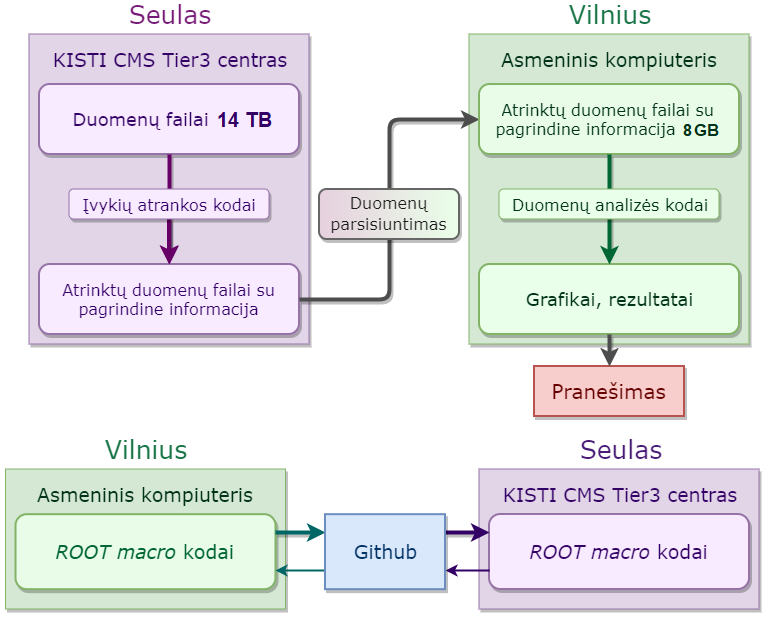
\includegraphics[width=0.7\textwidth]{Duomenu_panaudojimo_schema.png}
	\captionof{figure}{\label{fig:duomVald} Duomenų panaudojimo (viršuje) ir kompiuterinio kodo versijų valdymo (apačioje) schemos.}
\end{figure}

\begin{figure}[H]
	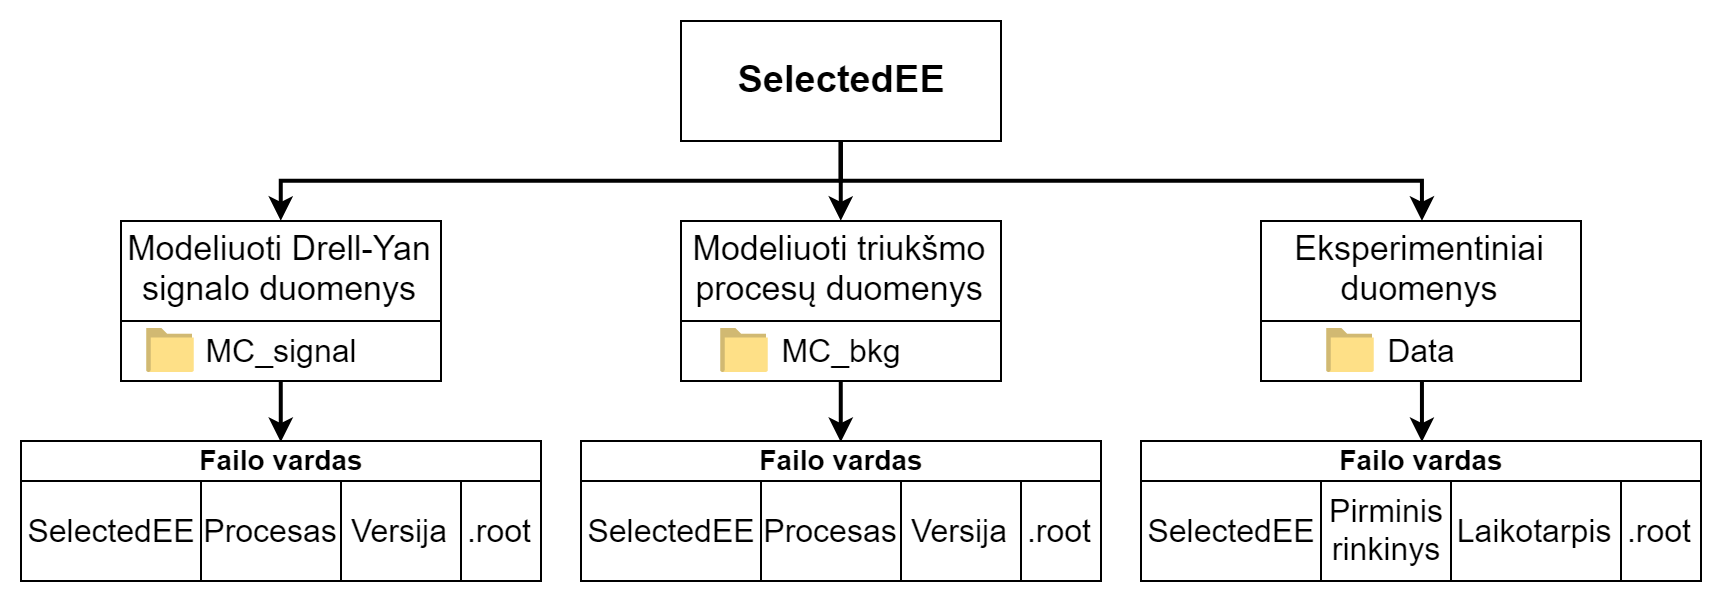
\includegraphics[width=\textwidth]{atrinktu_duomenu_schema_v1.png}
	\captionof{figure}{\label{fig:selectedX} Atrinktų duomenų loginė schema.}
\end{figure}

Duomenų analizė vykdyta dviem etapais: pirmiausia buvo atliekama išmatuotų ir modeliuotų įvykių atranka nuotoliniu
būdu prisijungus prie skaičiavimo centro.
Svarbiausia su atrinktais įvykiais susijusi informacija buvo įrašoma į naujus duomenų failus, kurie užima tik
apie $8$ GB.
Naujai sukurti failai buvo parsisiunčiami į vietinį kompiuterį tolimesnei analizei.
Sumažinti duomenų rinkiniai buvo skirstomi pagal tai, kokios galutinės būsenos įvykiai juose yra saugomi
($ee$, $\mu\mu$, ar $\emu$), tada pagal tai, ar įvykiai yra užregistruoti CMS detektoriumi, ar tai yra modeliuotas
Drell-Yan signalas, ar modeliuotas triukšmas.
Galiausiai atrinkti eksperimentinių duomenų failai buvo išskirstyti pagal pirmojo lygio trigerį ir įvykių
registravimo laikotarpį, o modeliuoti duomenų failai -- pagal procesą (bei, kai kuriais atvejais, tam tikrus
jo parametrus) ir failų versijas.
Sumažintų duomenų rinkinių loginio išdėstymo schema pateikta \ref{fig:selectedX} pav.
Programinio kodo versijos buvo tvarkomos naudojantis \textit{Github} versijų valdymo sistema.
Apibendrintos duomenų naudojimo ir kodo versijų valdymo schemos yra pavaizduotos \ref{fig:duomVald} pav.

\subsection{Įvykių atranka}\label{sec:selection}
Iš $2016$-aisiais metais CMS detektoriaus užregistruotų duomenų buvo stengiamasi išrinkti tokius įvykius, kurie
su kuo didesne tikimybe atitiktų Drell-Yan procesą.
Drell-Yan proceso miuonų galutinei būsenai buvo naudojamas vieno miuono trigeris, kuris aktyvuojamas tada,
kai aptinkamas bent vienas miuonas su skersiniu impulsu, didesniu nei $24$ GeV.
Miuonas turi būti atpažintas pasinaudojant trekų detektoriaus ir miuonų detektorių informacija.
Toliau kiekvienam miuonui buvo taikomi \ttt{TightID} reikalavimai \cite{MuonID}, kurie skirti sumažinti atranką
praeinančių netikrų miuonų, bei miuonų, atsiradusių iš antrinių procesų, skaičių.
\ttt{TightID} reikalavimus atitinka virš $95\%$ protonų susidūrimų metu sukurtų tikrų ir mažiau nei $0.3\%$ netikrų
miuonų \cite{MuonID}.
Taip pat kiekvienam miuonui buvo taikomas trajektorijos izoliuotumo reikalavimas: pašalinių dalelių, aptiktų
$\Delta R = \sqrt{(\Delta\eta)^2 + (\Delta\phi)^2} < 0.3$ (čia $\eta$ -- pseudosparta, $\phi$ -- sferinės koordinačių
sistemos azimutinis kampas) pločio kūgyje, nubrėžtame aplink miuono trajektoriją, skersinių impulsų suma negali
viršyti $15\%$ miuono skersinio impulso vertės.
Tolimesnis kriterijus buvo toks, kad miuonų poros trajektorijas pakankamai tiksliai eitų suvesti į vieną pirminę
viršūnę bei kad abu miuonai būtų priešingų elektrinių krūvių.
Tam, kad būtų išvengta miuonų iš kosminės spinduliuotės aptikimo, buvo taikomas papildomas kriterijus, reikalaujantis,
kad plokštuminis kampas tarp dviejų miuonų trajektorijų būtų mažesnis, nei $\pi-0.005$ rad.

Elektronų galutinei būsenai buvo naudojamas dviejų elektronų trigeris, kuris aktyvuojamas tada, kai aptinkami
bent du elektronai, vieno iš kurių skersinis impulsas didesnis, nei $23$ GeV, o kito -- didesnis nei $12$ GeV.
Kiekvienam elektronui buvo taikomi \ttt{MediumID} reikalavimai (idėja aprašyta \cite{EleID}, tačiau tikslios
reikalavimų vertės skiriasi nuo naudotų darbe, nes jos yra atnaujinamos CMS vidiniuose dokumentuose), kurie
skirti sumažinti elektronų, atsiradusių fotono virsmo į elektrono-pozitrono porą metu, bei netikrų elektronų
skaičių.
\ttt{MediumID} reikalavimus atitinka virš $80\%$ protonų susidūrimų metu sukurtų tikrų ir mažiau nei $3.5\%$ netikrų
elektronų \cite{EleID}.
Taip pat buvo reikalaujama, kad elektronai nepatektų į sritį $1.4442<|\eta_{\mathrm{SC}}|<1.566$, nes joje
yra perėjimas iš elektromagnetinio kalorimetro cilindrinės į antgalio dalį ir dėl ten išvedžiotos elektronikos
detektavimo efektyvumas šioje srityje nėra toks geras.

Galiausiai tiek elektronai, tiek miuonai turėjo praeiti tokius pačius kinematinius atrankos kriterijus,
reikalaujančius, kad greitesnysis leptonas turėtų skersinį impulsą, didesnį už $28$ GeV, o lėtesnysis --
didesnį už $17$ GeV bei kad abiejų leptonų pseudospartų absoliutinės vertės neviršytų $2.4$.
Jei tokią atranką praeitų kelios miuonų poros, iš jų išrenkama ta pora, kurių trajektorijas galima suvesti į
vieną pirminę viršūnę didžiausiu tikslumu.

Pagrindinis matuojamas dydis buvo atranką praėjusių leptonų porų invariantinė masė.
Iš jų verčių buvo brėžiama invariantinės masės histograma, apimanti masės sritį nuo $15$ iki $3000$ GeV.


\subsection{Pataisos}\label{sec:corrections}
CMS eksperimento matavimo rezultatų interpretavimui pasitelkiami modeliuoti protonų susidūrimai.
Matavime užregistruotų įvykių skaičius yra fiksuotas ir nulemtas integruotojo šviesio bei skirtingų
procesų reakcijų skerspjūvių.
Modeliuotų įvykių skaičius gali būti įvairus ir bendru atveju nesutampa su eksperimente užregistruotu
įvykių skaičiumi.
Kad būtų galima palyginti matavimą su modeliavimu, modeliuotų įvykių skaičius turi būti sunormuotas
į išmatuotą integruotąjį šviesį.
Tai daroma kiekvienam modeliuotam įvykiui priskiriant normuojantį svorį $\omega_{i}^{\mathrm{Norm.}}$,
kuris apskaičiuojamas pagal tokią formulę:
\begin{equation}
	\omega_{i}^{\mathrm{Norm.}} = \omega_{i}^{\mathrm{Gen.}} \frac{ \sigma\Lumi }{ \sum_{i=j}^{N}\omega_{j}^{\mathrm{Gen.}} } \; ,
	\label{eq:NLOweight}
\end{equation}
čia $\omega_{i}^{\mathrm{Gen.}}$ kiekvieno įvykio individualus svoris, priskirtas įvykių modeliavimo programos,
$\sigma$ -- tam tikro proceso (pvz., Drell-Yan) reakcijos skerspjūvis, $N$ -- įvykių skaičius to
proceso modeliuotų duomenų rinkinyje, $\Lumi$ -- išmatuotas integruotasis šviesis.
Daugumos procesų $\omega_{i}^{\mathrm{Norm.}}<1$.

Įprastai per vieną protonų spindulio paketų prasikeitimą (angl.\ \textit{bunch crossing}) susiduria
daugiau negu viena protonų pora ir tai turi įtakos užregistruoto įvykio atkūrimo kokybei.
Šį efektą bandoma simuliuoti modeliuotuose įvykiuose, tačiau dažniausiai tikimybinis protonų susidūrimų
skaičiaus (per vieną prasikeitimą) pasiskirstymas matavime ir modeliavime nesutampa.
Tai siejasi su atsitiktinėmis susidūrimų fliuktuacijmis, o taip pat ir su Didžiojo hadronų greitintuvo
technikų tyrinėjimais keičiant protonų spindulio intensyvumą, paketų skaičių, spindulio persiklojimo
tūrį ir pan.
Šį nesutapimą bandoma sumažinti taikant protonų susidūrimo skaičiaus pataisas -- kiekvienam modeliuotam
įvykiui priskiriamas tam tikras papildomas svoris pagal tai, koks protonų susidūrimų skaičius jame buvo sumodeliuotas.
Pataisa buvo taikoma darant prielaidą, kad protonų susidūrimo skerspjūvis greitintuve yra lygus $64$ mb
($6.4 \cdot 10^{-30} \, \mathrm{m}^2)$.
Išmatuoti ir modeliuoti atkurtų pirminių viršūnių skaičiaus pasiskirstymai elektronų poros įvykiuose
prieš ir po pataisos pateikiami \ref{fig:PUba} pav.
Miuonų poros įvykiams grafikų forma yra analogiška, tik skiriasi suminis įvykių skaičius.

Paveikslų apatinėse dalyje pateiktuose eksperimentinio ir modeliuoto rezultatų santykio grafikuose galima pamatyti, kad
$10$-$30$ pirminių viršūnių skaičiaus srityje, į kurią patenka apie $91\%$ visų įvykių, grafikai tampa plokštesni --
šioje srityje pirminių viršūnių skaičiaus pasiskirstymai sutampa labai gerai (skirtumas $\leqslant 9\%$).

Elektronų poros invariantinės masės matavimo kokybei ženklios įtakos turi elektronų energijos matavimo
tikslumas, o miuonų poros invariantinei masei -- miuonų skersinio impulso matavimo tikslumas.
Dėl to visiems užregistruotiems elektronams buvo pritaikytos standartinės CMS elektronų energijos skalės
pataisų procedūros \cite{Ecorr}, o miuonams -- Ročesterio mokslinės grupės pateikiamos miuonų impulso
skalės pataisos \cite{RocCorr}.

\begin{figure}[tbp]
	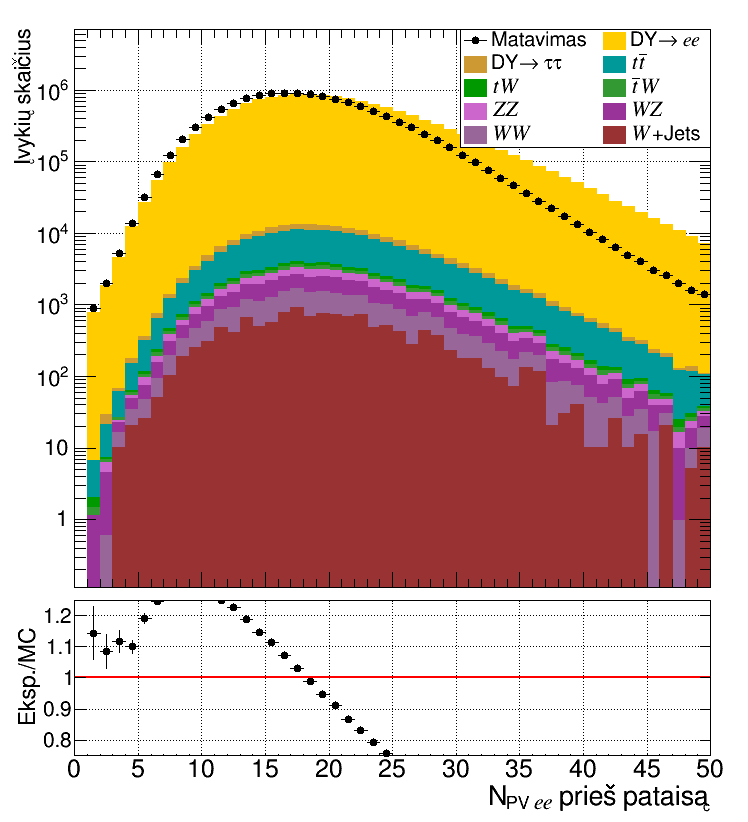
\includegraphics[width=0.48\textwidth]{nVTXee_before.png}
	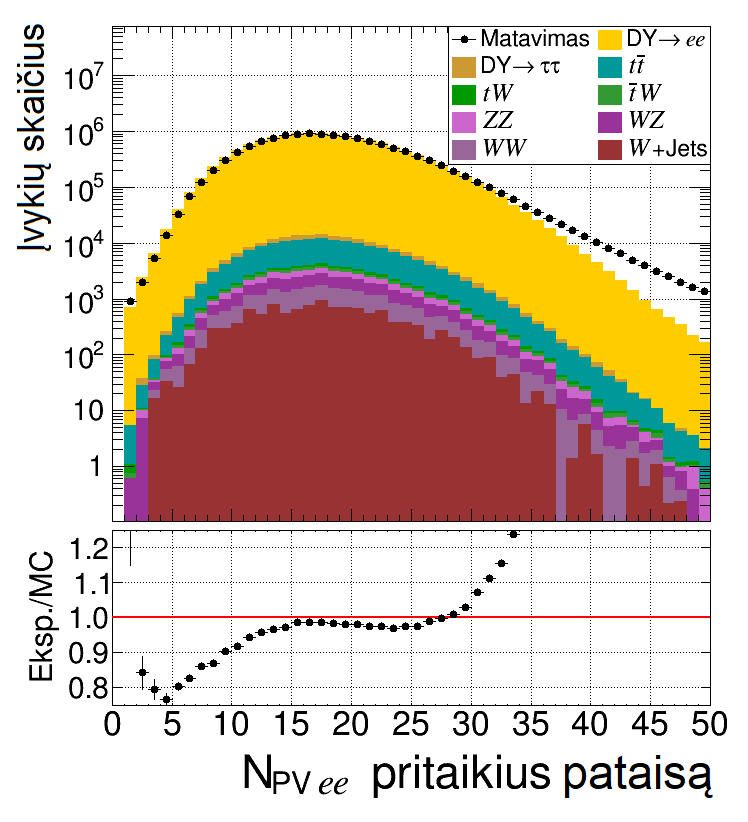
\includegraphics[width=0.48\textwidth]{nVTXee_after.png}
	\caption{\label{fig:PUba} Pirminių viršūnių skaičiaus pasiskirstymai atranką praėjusiuose elektronų poros
		įvykiuose prieš (kairėje) ir po (dešinėje) pataisos pritaikymo.
		Juodi taškai vaizduoja CMS detektoriumi išmatuotą, o spalvoti stulpeliai -- modeliuotus pasiskirstymus.}
\end{figure}

\begin{figure}[tbp]
	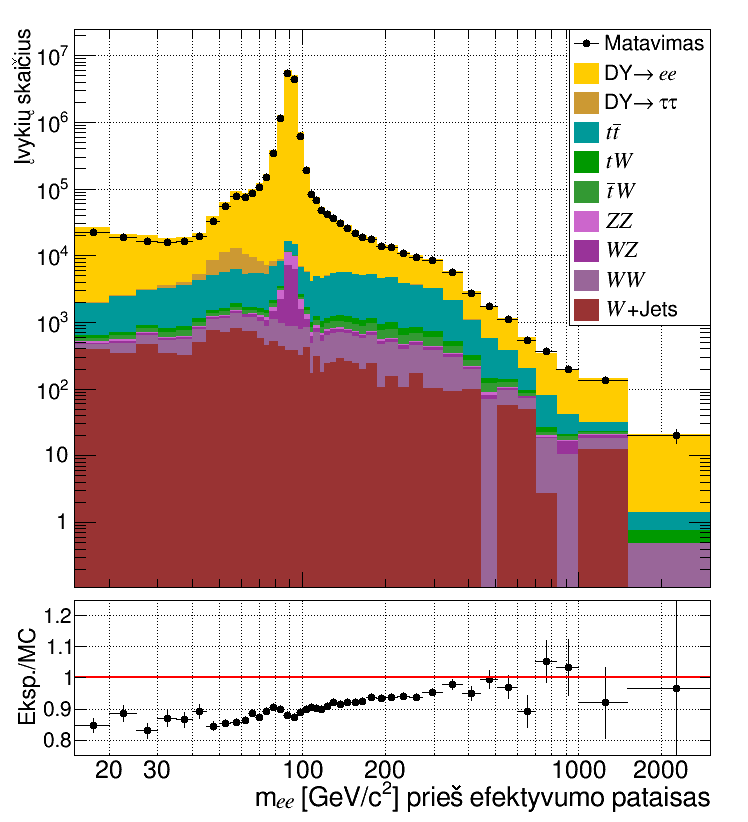
\includegraphics[width=0.48\textwidth]{ee_mass_beforeSF.png}
	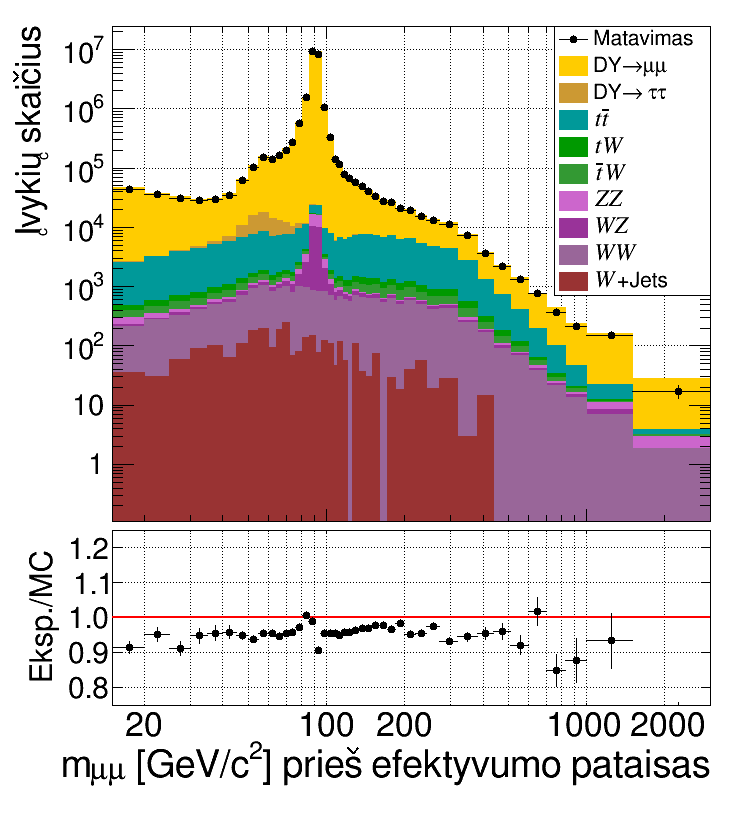
\includegraphics[width=0.48\textwidth]{mumu_mass_beforeSF.png}
	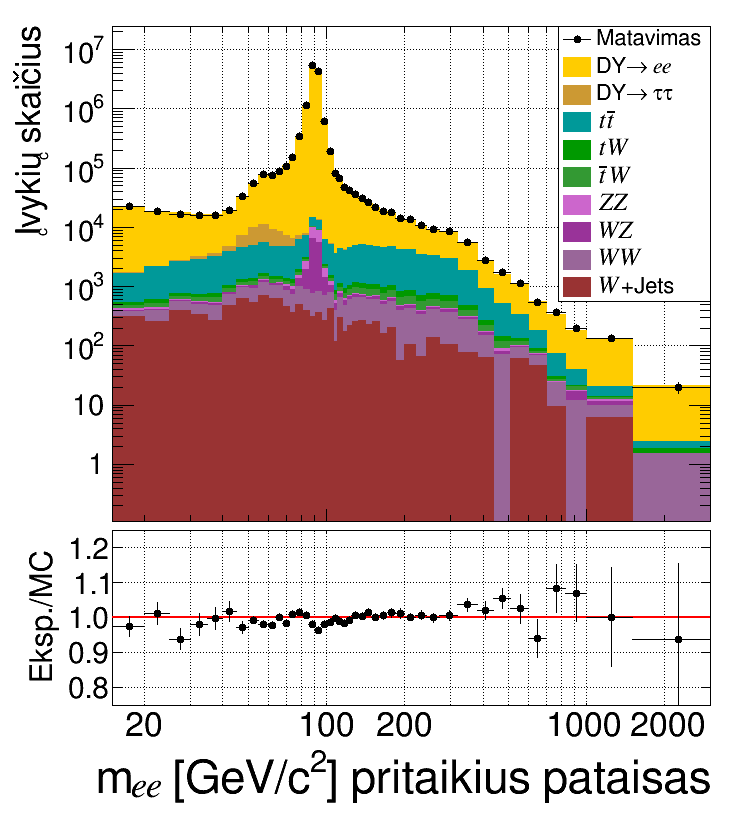
\includegraphics[width=0.48\textwidth]{ee_mass_after.png}
	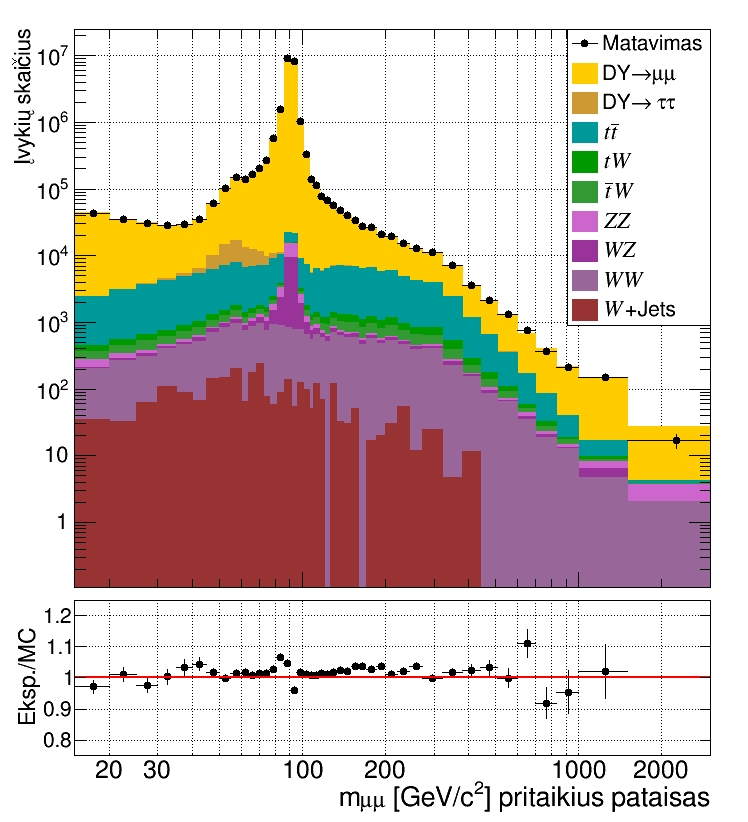
\includegraphics[width=0.48\textwidth]{mumu_mass_after.png}
	\caption{\label{fig:invMba} Elektronų (kairėje) ir miuonų (dešinėje) porų invariantinės masės pasiskirstymai
		prieš (viršuje) ir po (apačioje) efektyvumo pataisų pritaikymo.}
\end{figure}

Kadangi dėl modeliavimo netobulumo nesutapo tam tikros realaus ir virtualaus eksperimento sąlygos,
kiekvienam elektronų poros įvykiui buvo priskiriami svoriniai daugikliai, priartinantys modeliuotus trigerių
suveikimo ir elektrono trajektorijos atkūrimo bei atpažinimo efektyvumus prie išmatuotųjų verčių.
Miuonų poros įvykiams buvo priskirti daugikliai, atsižvelgiantys į trigerių bei miuonų trajektorijos atkūrimo,
atpažinimo ir izoliuotumo įvertinimo efektyvumų nesutapimus.
Kiekvieno suvidurkinto daugiklio vertė buvo nustatoma pagal leptono skersinio impulso ir pseudospartos vertes.
Tipinė daugiklio vertė yra apie $0.9$.
Invariantinės masės pasiskirstymai prieš ir po šių pataisų pritaikymo pateikiami atitinkamai \ref{fig:invMba} pav.
Palyginus paveikslų apačioje pateikiamus matavimo ir modeliavimo santykio pasiskirstymus galima pamatyti, kad
pritaikius minėtas pataisas sutapimas tarp eksperimento ir modeliavimo pagerėjo vidutiniškai apie $10\%$.

Yra pastebėta, kad pirmos eilės perturbacijų tikslumu modeliuojant viršūninių kvarkų poros ($t\bar{t}\,$)
įvykius, gaunami modeliuoti viršūninių kvarkų skersinių impulsų pasiskirstymai turi nesutapimų su nustatytaisiais
eksperimentiškai \cite{ttbarPT}.
Kadangi $t\bar{t}$ yra vienas iš Drell-Yan triukšmo procesų, norint turėti kuo tikslesnį triukšmo įvertį, į šį
modeliavimo trūkumą svarbu atsižvelgti.
Tai buvo daroma modeliuotiems viršūninių kvarkų poros įvykiams priskiriant papildomus svorius, kurie skirti
priartinti modeliuotą kvarkų skersinių impulsų pasiskirstymą prie naujausių eksperimentinių rezultatų.
Svorių vertės nustatomos pagal kvarkų skersinių impulsų $p_{\mathrm{T}}^{t}$ vertes.
Tipinės svorių vertės $>1$, kai abiejų kvarkų $p_{\mathrm{T}}^{t}<123 \, \mathrm{GeV}$, ir $<1$,
kai $p_{\mathrm{T}}^{t}>120 \, \mathrm{GeV}$.

Neidealios eksperimentinės sąlygos nulemia matavimo ir modeliavimo rezultatų nesutapimą.
Dvi aplinkybės paveikė leptonų poros spartos pasiskirstymus.
Į tai atsižvelgti modeliuotiems įvykiams buvo pritaikytos dvi papildomos pataisos.
Viena pataisa buvo skirta ištaisyti protonų susidūrimo vietos $z$ koordinatės ($z$ ašis eina išilgai protonų
spindulio lėkimo krypties detektoriaus centre) nesutapimą tarp matavimo ir modeliavimo.
Tai padėjo sumažinti \ref{fig:rapibPVZ} pav.\ apačioje esančiuose matavimo ir modeliavimo santykio pasiskirstymuose
matomus asimetriškumus.
Kita pataisa buvo reikalinga todėl, kad darbe naudotų duomenų registravimo laikotarpiu buvo susidurta su problema,
kai tam tikru atveju trigerio suveikimas buvo priskiriamas ne tam įvykiui, kuris iš tikrųjų jį aktyvavo, o
ankstesniam.
Dėl šio efekto dalis įdomių įvykių, kuriuose sukurtos dalelės turėjo dideles pseudospartos vertes ($|\eta|>2$)
liko neįrašyti.
Imituoti šiam pernelyg ankstyvo trigerio suveikimo efektui buvo pritaikyta pataisa, kuri priskirdavo įvykiams
svorius pagal tai, kiek ir kokių įvykyje užregistruotų objektų patenka į didesnių pseudospartų sritį.
Tai turėjo įtakos ir leptonų poros spartos pasiskirstymui: palyginus \ref{fig:rapibL1} su \ref{fig:rapia} pav.\
galima matyti, kad pataisos pritaikymas padėjo sumažinti modeliuotų įvykių skaičių ties didesnėmis spartos modulio
vertėmis ir priartino modeliuotus rezultatus prie išmatuotųjų.
Tipinės pataisų vertės vienam įvykiui siekė apie $0.98$ ir mažiau įvykiams, kuriuose buvo užfiksuoti objektai su
$|\eta|>2$.

\begin{figure}[H]
	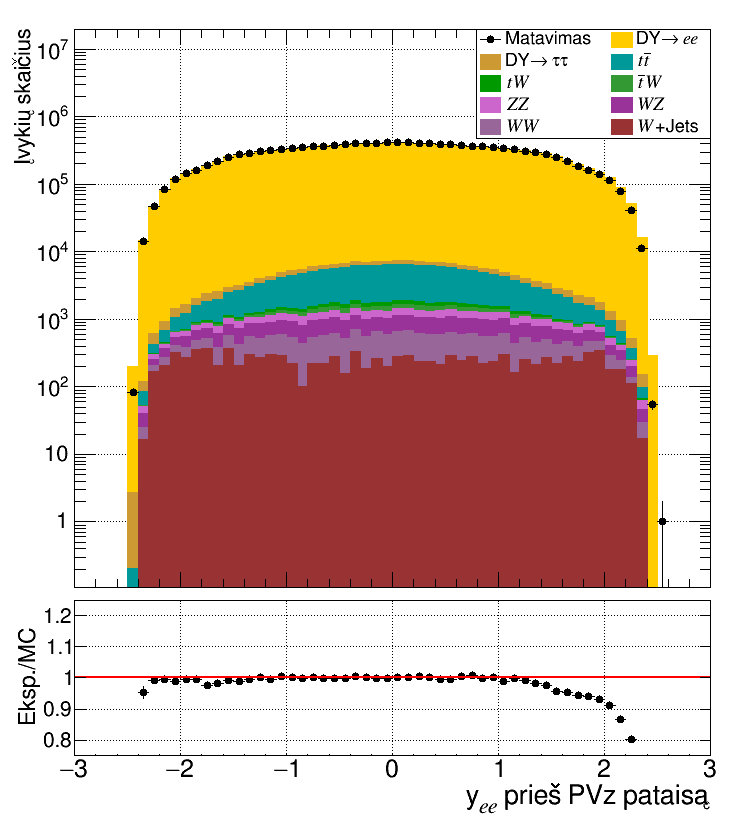
\includegraphics[width=0.48\textwidth]{ee_rapi_beforePVZ.png}
	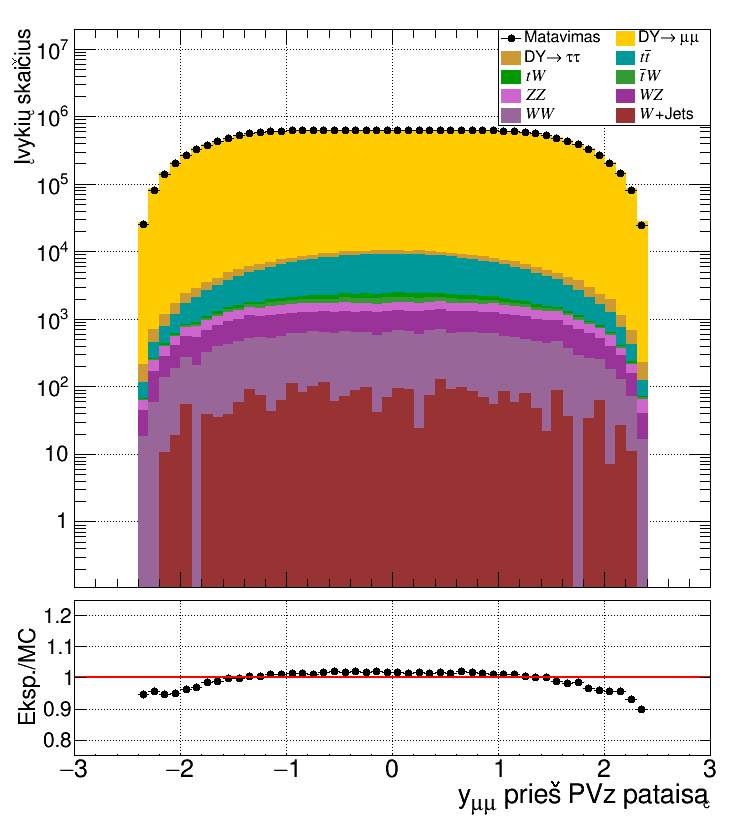
\includegraphics[width=0.48\textwidth]{mumu_rapi_beforePVZ.png}
	\caption{\label{fig:rapibPVZ} Elektronų (kairėje) ir miuonų (dešinėje) porų spartos pasiskirstymai
		prieš pirminės viršūnės $z$ koordinatės pataisos pritaikymą.
		Atkreiptinas dėmesys į eksperimento ir modeliavimo santykio pasiskirstymo asimetriškumą.}
\end{figure}

\begin{figure}[H]
	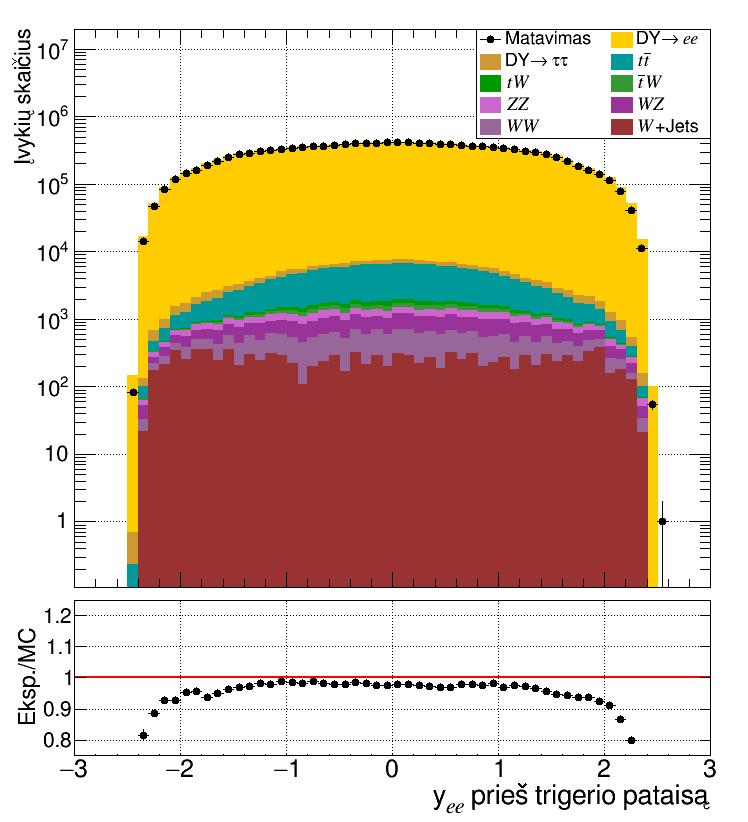
\includegraphics[width=0.48\textwidth]{ee_rapi_beforeL1.png}
	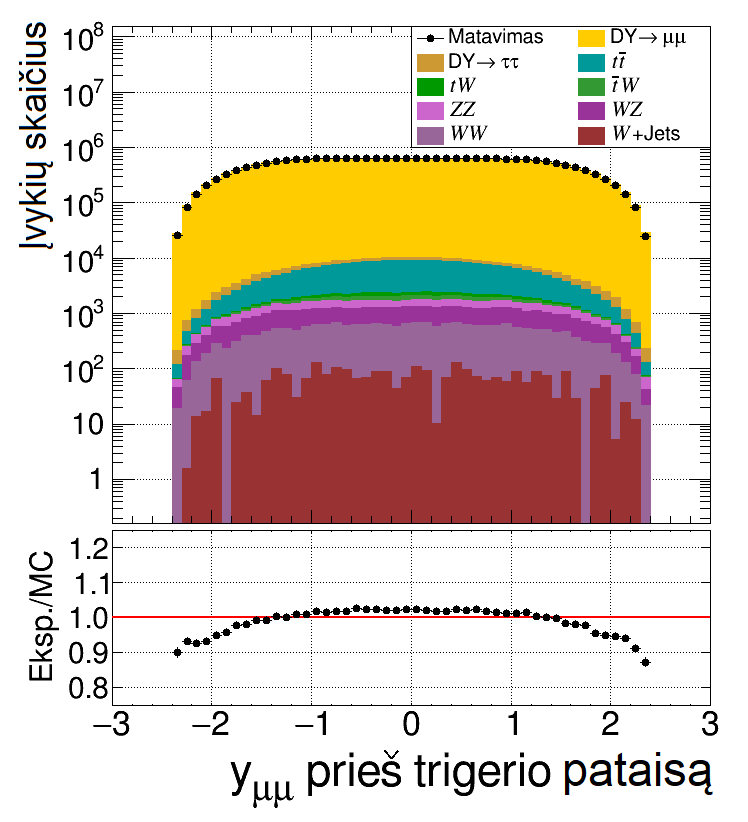
\includegraphics[width=0.48\textwidth]{mumu_rapi_beforeL1.png}
	\caption{\label{fig:rapibL1} Elektronų (kairėje) ir miuonų (dešinėje) porų spartos pasiskirstymai,
		gauti po pirminės viršūnės $z$ koordinatės pataisos pritaikymo, tačiau dar nepritaikius per ankstaus
		trigerio suveikimo pataisos.}
\end{figure}

\begin{figure}[H]
	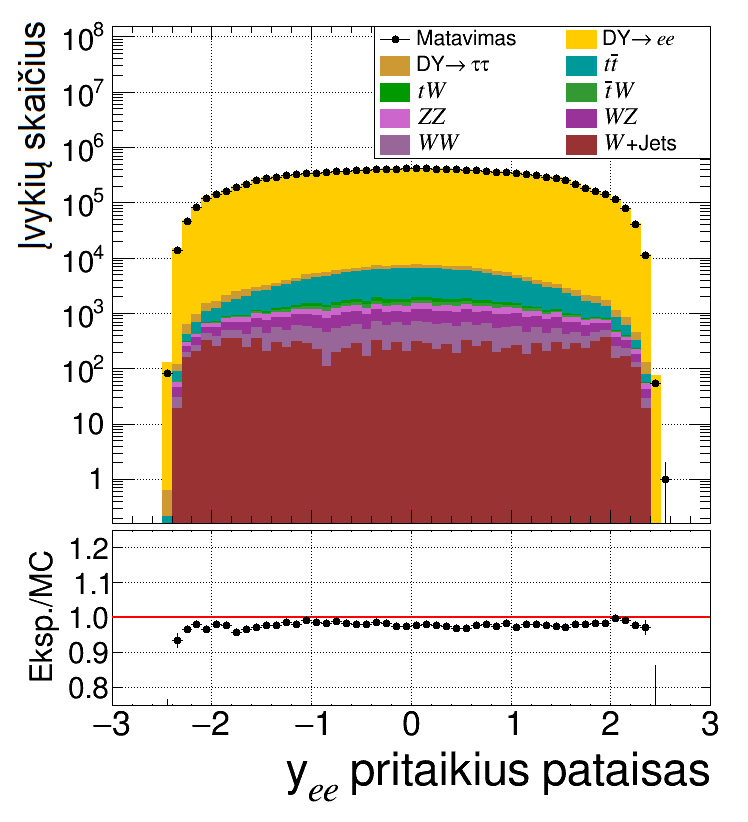
\includegraphics[width=0.48\textwidth]{ee_rapi_after.png}
	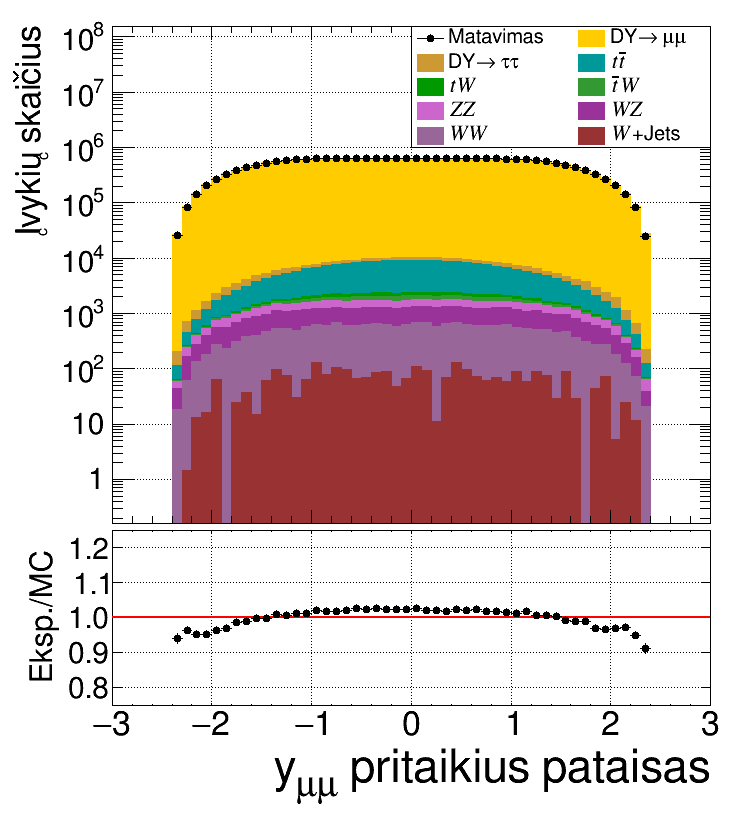
\includegraphics[width=0.48\textwidth]{mumu_rapi_after.png}
	\caption{\label{fig:rapia} Elektronų (kairėje) ir miuonų (dešinėje) porų spartos pasiskirstymai,
		gauti pritaikius visas pataisas.}
\end{figure}

\subsection{Triukšmų indėlio įvertinimas}\label{sec:SignalBkg}

$\emu$ metodu buvo įvertinti šie triukšmai: $\DYtau$, $t\bar{t}\,$, $WW$, $tW$, $\bar{t}W$.
Kitų triukšmo procesų indėlis buvo įvertintas modeliavimu, išskyrus $QCD$ įvykius, kurių modeliavimas neaprašo pakankamai
gerai.
Ateityje $QCD$ indėlis bus įvertintas klaidingo atpažinimo metodu, o į dabartinį tyrimą jis nebuvo įtrauktas.

Taikant $\emu$ metodą signalo sritis apibrėžiama pagal \ref{sec:selection} skyriuje aprašytus kriterijus.
Kontrolinė sritis apibrėžiama pagal panašius kriterijus, tačiau galutinėje būsenoje ieškome
ne dviejų elektronų ar dviejų miuonų, o vieno elektrono ir vieno miuono.
Tokios būsenos neįmanoma gauti iš Drell-Yan proceso signalo, taigi joje bus vien triukšmo įvykiai.
Triukšmo įvykių skaičius iš kontrolinės srities ($\emu$) į signalo sritį ($ee$ arba $\mu\mu$)
transformuojamas pasinaudojant Monte Carlo modeliavimo rezultatais:

\begin{equation}
	N_{ee}^{\mathrm{Tr. \, įvert.}} =
	\frac{ N_{ee}^{\mathrm{Tr. \, MC}} }{ N_{e\mu}^{\mathrm{Tr. \, MC}} }
	\cdot N_{e\mu}^{\mathrm{Tr. \, eksp.}} \; ,
	\label{eq:emuMethod}
\end{equation}
čia $N_{ee}^{\mathrm{Tr. \, įvert.}}$ -- $\emu$ metodu įvertintas triukšmo įvykių skaičius signalo
(šiuo atveju, $ee$) srityje, $N_{e\mu}^{\mathrm{Tr. \, eksp.}}$ -- išmatuotas įvykių skaičius
kontrolinėje srityje, $N_{ee}^{\mathrm{Tr. \, MC}}$ ir $N_{e\mu}^{\mathrm{Tr. \, MC}}$ -- modeliuotų
triukšmo įvykių skaičiai atitinkamai signalo ir kontrolinėje srityje.

Elektrono ir miuono galutinės būsenos įvykiai buvo atrenkami kombinuojant $ee$ ir $\mu\mu$ atrankos
kriterijus -- elektronui buvo taikomi $ee$ atrankoje naudoti, o miuonui -- $\mu\mu$ atrankoje naudoti
kriterijai, tik šiai atrankai buvo naudotas vieno miuono trigeris (nenaudota elektronų trigerių).
Šiems įvykiams buvo pritaikytos ir visos \ref{sec:corrections} skyriuje aprašytos pataisos.

Kadangi $\emu$ įvykių atranką praeina ir ganėtinai reikšminga netikrų $\emu$ įvykių dalis (pagrinde
$W+\mathrm{Jets}$ ir $QCD$ įvykiai, kuriuose čiurkšlė būna klaidingai atpažinta kaip leptonas),
norint kaip įmanoma tiksliau įvertinti Drell-Yan proceso triukšmus, pirmiausia reikia
įvertinti netikrų $\emu$ įvykių skaičių.
$QCD$ indėlis buvo įvertintas dar vienu matavimu grįstu metodu.
Šiuo atveju signalo sritis buvo $\emu$ įvykiai, kuriuose elektronas ir miuonas yra priešingų elektrinių
krūvių, o kontrolinė sritis -- įvykiai, kuriuose elektrono ir miuono krūviai yra vienodi.
$QCD$ įvykių skaičiaus įvertinimo principas yra pavaizduotas \ref{fig:emuQCD} pav.
Kairiajame grafike matomas didžiulis skirtumas tarp eksperimentinio ir modeliuoto rezultato buvo
priskirtas su $QCD$ procesu siejamiems netikriems $\emu$ įvykiams.
$QCD$ įvykių skaičius iš vienodų krūvių (kontrolinės) srities į priešingų krūvių (signalo) sritį
buvo transformuotas padalinus jį iš konstantos $R\approx 0.57$, kuri apskaičiuojama teoriškai,
padarius prielaidą, kad visi atranką praeinantys $QCD$ įvykiai yra gelminių kvarkų poros
($b\bar{b}$) įvykiai.
$W+\mathrm{Jets}$ indėlis buvo įvertintas iš modeliavimo.
Prieš taikant $\emu$ metodą gautas netikrų $\emu$ įvykių skaičiaus įvertis buvo atimtas iš
$N_{e\mu}^{\mathrm{Tr. \, eksp.}}$, o $W+\mathrm{Jets}$ indėlis buvo įskaitytas sumažinant
$N_{e\mu}^{\mathrm{Tr. \, eksp.}}$ dydžiu $1/(1+C)$, kur
\begin{equation*}
	C = \frac{ N_{W+\mathrm{Jets}}^{\mathrm{MC}} } { N_{\mathrm{DY}\rightarrow\tau\tau}^{\mathrm{MC}} + 
	N_{t\bar{t}}^{\mathrm{MC}} + N_{WW}^{\mathrm{MC}} + N_{WZ}^{\mathrm{MC}} + N_{tW}^{\mathrm{MC}} + N_{\bar{t}W}^{\mathrm{MC}} +
	N_{ZZ}^{\mathrm{MC}} } \; ,
\end{equation*}
čia $N^{\mathrm{MC}}_{\mathrm{proc.}}$ -- modeliuotų tam tikro proceso $\emu$ galutinės būsenos įvykių skaičius.

\begin{figure}[H]
	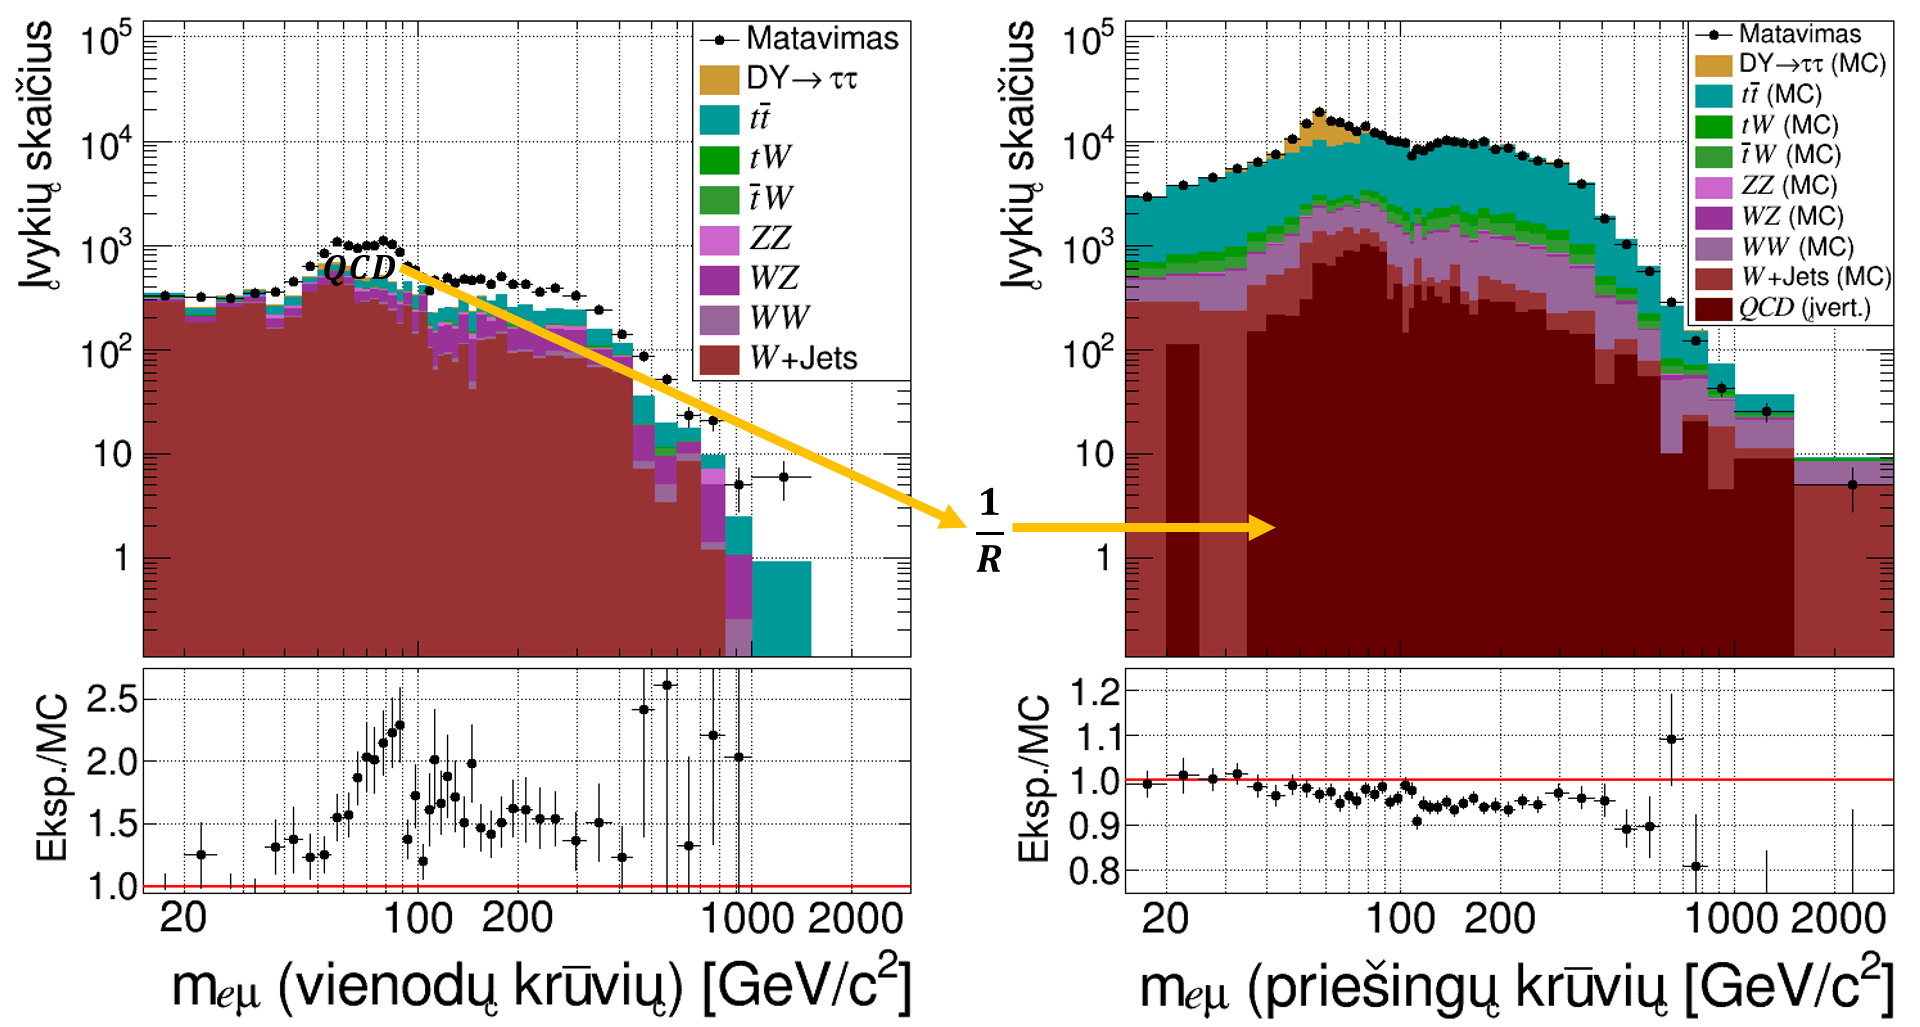
\includegraphics[width=0.95\textwidth]{emuQCDest.png}
	\vspace{-0.2cm}
	\caption{\label{fig:emuQCD} Vienodą (kairėje) ir priešingą (dešinėje) krūvį turinčių elektrono ir
	miuono invariantinės masės pasiskirstymai.
	Rodyklės iliustruoja, kaip buvo įvertinamas netikrų $\emu$ ($QCD$) įvykių skaičius.
	}
\end{figure}

\vspace{-1cm}
\subsection{Paklaidų įvertinimas}\label{sec:uncertainties}
\vspace{-0.2cm}

Analizuojant $pp$ susidūrimus laikoma, kad procesai yra pasiskirstę pagal Puasono dėsnį.
Puasono pasiskirstymu aprašomų įvykių skaičiaus standartinis nuokrypis yra lygus kvadratiniai šakniai iš labiausiai
tikėtino įvykių skaičiaus.
Vis dėlto, labiausiai tikėtinas įvykių skaičius nėra žinomas dydis, todėl atranką praėjusių įvykių skaičiaus neapibrėžtumo
vertė yra gaunama ištraukus kvadratinę šaknį iš turimo įvykių skaičiaus.

Kai modeliuoti įvykiai turi nelygius vienetui svorius, jų skaičiaus neapibrėžtumas skaičiuojamas ištraukiant
kvadratinę šaknį iš modeliuotų įvykių svorių kvadratų sumos:
\begin{equation}
	(\Delta N)_{\mathrm{Stat.\,}} = \sqrt{\sum_{i=1}^{N}w_{i}^{2}} \; ,
	\label{eq:Sumw2Unc}
\end{equation}
čia $$w_{i}=w_{i}^{\mathrm{Norm.}} \cdot \prod_{p=1}^{N_{\mathrm{Pat.}}}w_{i \, p} \; ,$$
kur $w_{i}^{\mathrm{Norm.}}$ -- modeliuoto įvykio normuojantis svoris, $w_{i \, p}$ -- modeliuotam įvykiui priskirtas
tam tikros pataisos $p$ svorinis daugiklis, $N_{\mathrm{Pat.}}$ -- pataisų skaičius.
Į \eqref{eq:Sumw2Unc} formulę įstačius vienetinius svorius (eksperimentiniai įvykiai) gauname, kad tokiu atveju įvykių
skaičiaus paklaida lygi jau minėtajai kvadratinei šakniai iš įvykių skaičiaus.

Kai įvykių skaičius yra išvestinis dydis (pavyzdžiui,  apskaičiuotas pagal \eqref{eq:emuMethod} formulę) jo neapibrėžtumas
 apskaičiuojamas pasinaudojant šia išraiška:

\begin{equation}
	\Delta f(x, y, ...) =
	\sqrt{ \left( \frac{\partial f}{\partial x} \Delta x \right)^{2} +
	\left( \frac{\partial f}{\partial y} \Delta y \right)^{2} + ... } \;\; \mathrm{,}
	\label{eq:DerUnc}
\end{equation}
čia $x$ ir $y$ -- nepriklausomi dydžiai.

Galimiems sisteminiams nukrypimams įvertinti CMS statistikos komitetas rekomenduoja turėti bent du skirtingais būdais
atliktus matavimus, kurie, idealiu atveju, turėtų duoti panašų įvertį.
Kadangi tikroji vertė, kurią bandoma išmatuoti, yra nežinoma, daroma prielaida, jog atlikti skirtingi matavimai yra
lygiaverčiai, ir tikroji vertė yra artimoje aplinkoje.
Tokiu atveju saugu sistemine tam tikros išmatuotos vertės paklaida laikyti skirtumo tarp dviejų skirtingų matavimų
modulį.
Šiame darbe buvo matuojamas Drell-Yan proceso triukšmo įvykių skaičius, o turimi du skirtingi įverčiai -- modeliuotas ir
apskaičiuotas naudojant $\emu$ metodą.
Taigi, Drell-Yan proceso triukšmo įvykių skaičiaus sisteminė paklaida buvo įvertinta pagal tokią formulę:
\begin{equation}
	(\Delta N_{ll}^{\mathrm{Tr. \, įvert.}})_{\mathrm{Sist.\,}} = | N_{ll}^{\mathrm{Tr. \, įvert.}} -
	N_{ll}^{\mathrm{Tr. \, MC}} | \; .
	\label{eq:systUnc}
\end{equation}

\vspace{-1cm}
\section{Rezultatai ir jų aptarimas}
\vspace{-0.2cm}

Drell-Yan proceso triukšmo įvykių skaičius tiek $ee$, tiek $\mumu$ galutinėms būsenoms buvo įvertintas $\emu$
metodu ($\DYtau$, $t\bar{t}\,$, $WW$, $tW$, $\bar{t}W$ procesams) arba iš modeliavimo ($W+\mathrm{Jets}$, $WZ$,
$ZZ$ procesams).
$QCD$ triukšmo įvykių skaičius, patenkantis į $ee$ ir $\mu\mu$ sritis, kol kas įvertintas nebuvo.
$\emu$ metodas buvo taikomas kiekvienam histogramos stulpeliui atskirai, naudojantis \eqref{eq:emuMethod} formule.
Statistinės įvykių skaičiaus paklaidos buvo įvertintos naudojantis \eqref{eq:Sumw2Unc} ir \eqref{eq:DerUnc}
formulėmis, o sisteminės paklaidos -- naudojantis \eqref{eq:systUnc} formule.
Suminės paklaidos gautos susumavus statistinę ir sisteminę paklaidas pagal Pitagoro teoremą.
Triukšmo įvykių skaičiaus įverčiai, gauti $\emu$ metodu, pateikiami \ref{fig:bkgEst} pav.
Po grafikais taip pat pateikiami įverčio ir modeliavimo santykio pasiskirstymai.
Grafikuose juodi vertikalūs brūkšniai žymi statistines, o mėlynai užtušuotos juostos -- sumines įvykių skaičiaus paklaidas.
Tokio žymėjimo laikomasi visuose pateikiamuose grafikuose.
Visoje tirtoje invariantinių masių srityje susumuotas modeliuotų $ee$ triukšmo įvykių skaičius yra lygus $165031$,
o $e\mu$ metodu įvertintas $ee$ triukšmo įvykių skaičius lygus $158777$.
Modeliuotų $\mu\mu$ triukšmo įvykių skaičius lygus $250500$, o įvertinus $\mu\mu$ triukšmo įvykių skaičių  $e\mu$ metodu
gauta $241105$ įvykių.
Lyginant su modeliavimu, $\emu$ metodas visoje tirtoje invariantinės masės srityje susumuotą triukšmo įvykių skaičių
sumažino maždaug $4$-ais procentais.
Šis skirtumas yra sisteminė paklaida.
\ref{fig:bkgEst} pav. apačioje pateikti $\emu$ įverčio ir modeliavimo santykio grafikai atrodo taip pat
tiek $ee$, tiek $\mu\mu$ įvykiams, nes, pagal \eqref{eq:emuMethod} formulę,
$$\frac{N_{ll}^{\mathrm{Tr. \, įvert.}}}{N_{ll}^{\mathrm{Tr. \, MC}}} =
\frac{N_{\emu}^{\mathrm{Tr. \, eksp.}}}{N_{\emu}^{\mathrm{Tr. \, MC}}} \; .$$
Šis santykis yra vienodas tiek $ee$, tiek $\mu\mu$ įvykiams.

\ref{fig:MassDataMCest} pav. pateikiamos leptonų porų invariantinių masių histogramos, kuriose $\DYtau$, $\ttbar$,
$tW$, $\tbarW$, ir $WW$ procesų modeliuoti įverčiai yra pakeisti į gautuosius naudojant $\emu$ metodą (legendoje žymima
\ltq{įvert.}).
Šie triukšmo įvykiai sudaro $1.23\%$ visų $ee$ ir $1.06\%$ visų $\mu\mu$ įvykių.
Po grafikais pateikiami matavimo ir suminio (Drell-Yan signalo, $WW$, $ZZ$ ir $W+\mathrm{Jets}$ modeliuoto ir 
$e\mu$ metodu įvertinto kitų triukšmo procesų) įverčio santykio pasiskirstymai.

Nors $\emu$ metodas leido sėkmingai įvertinti Drell-Yan proceso triukšmo įvykių skaičių, ateityje metodiką
vertėtų patobulinti.
Tikslingiausia būtų pabandyti netikrų $\emu$ įvykių skaičių įvertinti kitais matavimu grįstais metodais.
Darbas bus tęsiamas bendradarbiaujant su CMS kolektyvo mokslininkais.

\begin{figure}[H]
	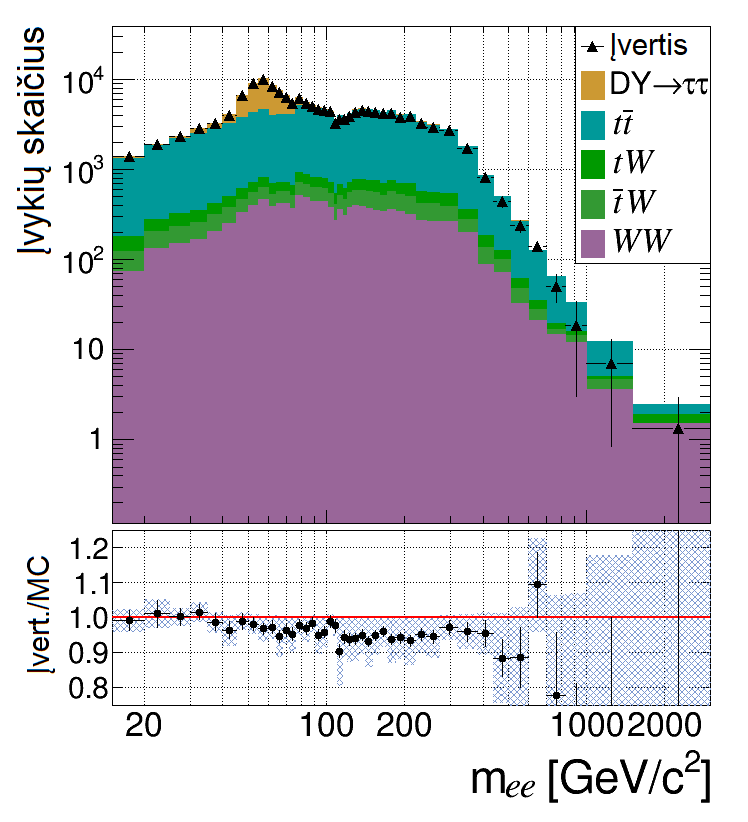
\includegraphics[width=0.49\textwidth]{ee_bkg_est.png}
	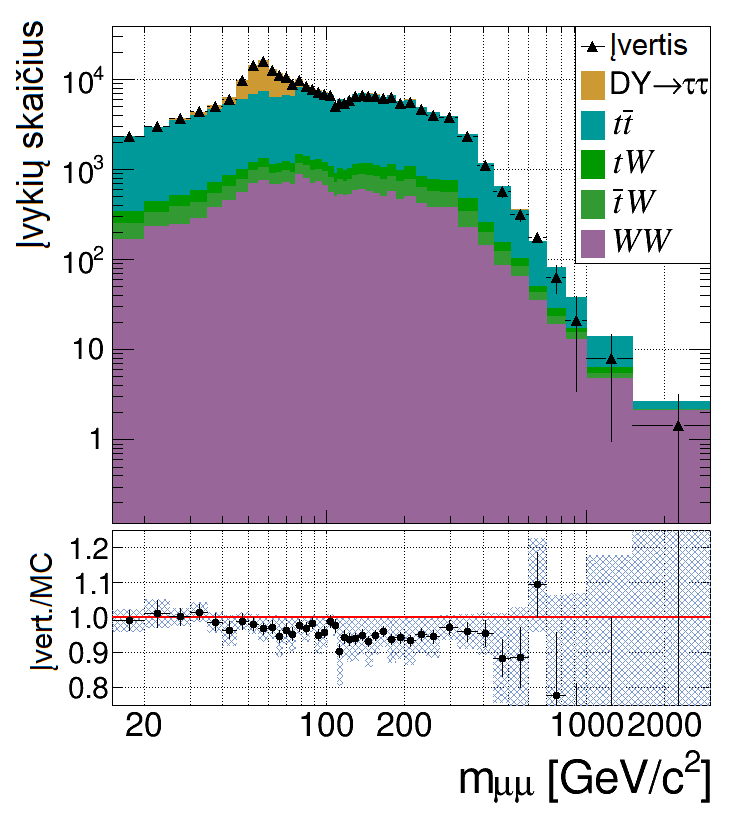
\includegraphics[width=0.49\textwidth]{mumu_bkg_est.png}
	\caption{\label{fig:bkgEst}
		Su Drell-Yan triukšmo procesais siejamų elektronų (kairėje) ir miuonų (dešinėje) porų invariantinių masių pasiskirstymai.
		Spalvoti histogramų stulpeliai vaizduoja modeliuotus, o juodi taškai -- $\emu$ metodu apskaičiuotus pasiskirstymus.}
\end{figure}

\begin{figure}[H]
	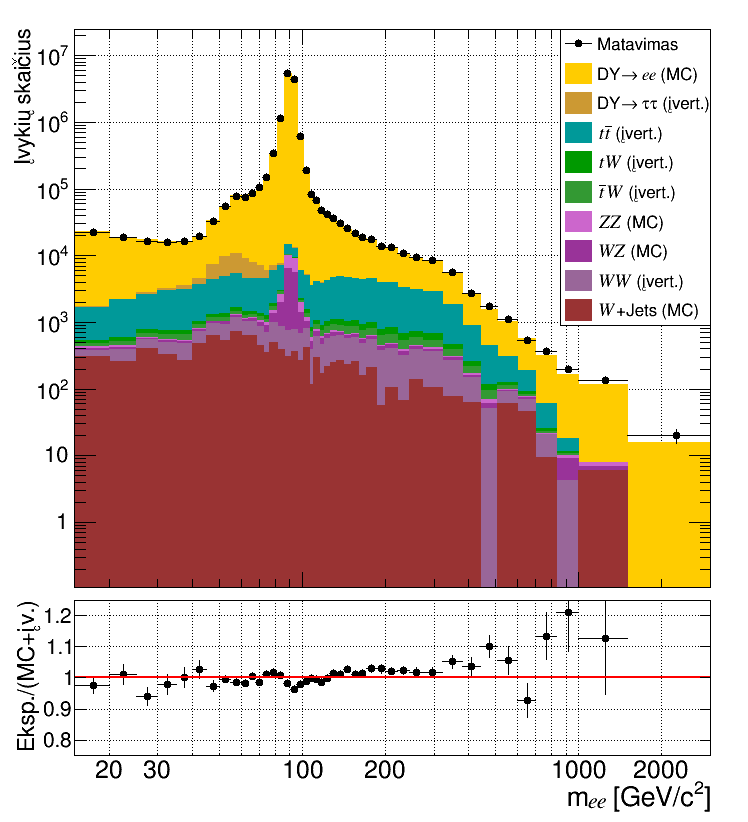
\includegraphics[width=0.49\textwidth]{ee_mass_est.png}
	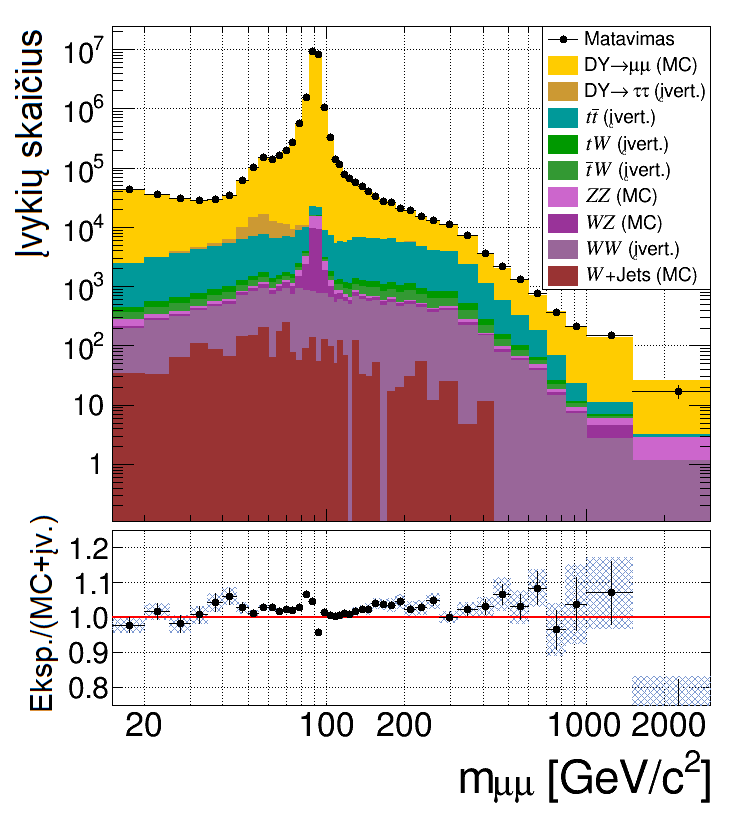
\includegraphics[width=0.49\textwidth]{mumu_mass_est.png}
	\caption{\label{fig:MassDataMCest}
		Elektronų (kairėje) ir miuonų (dešinėje) porų invariantinių masių pasiskirstymų histogramos.
		Juodi taškai vaizduoja CMS detektoriumi išmatuotą, o spalvoti stulpeliai -- modeliuotus ir $\emu$ metodu įvertintus
		pasiskirstymus.}
\end{figure}


\section{Išvados}
\begin{enumerate}
	\item Duomenų rinkinių sukūrimas, saugant tik atranką praėjusius įvykius, gerokai sutrumpina tolimesnės duomenų analizės
	laiką bei supaprastina duomenų saugojimą;
	\item Eksperimento ir modeliavimo sąlygų nesutapimų pataisos padeda sumažinti atranką praeinančių išmatuotų ir modeliuotų
	įvykių skaičiaus neatitikimus;
	\item Iš matavimo duomenų įvertinus su $QCD$ siejamų netikrų $\emu$ įvykių skaičių galima patikslinti tikrų $\emu$ įvykių
	skaičių, tačiau ateityje vertėtų pabandyti kitus matavimu grįstus metodus, leidžiančius įvertinti visų netikrų $\emu$
	įvykių skaičių (įskaitant ir $W+\mathrm{Jets}$);
	\item $\emu$ metodas yra tinkamas Drell-Yan proceso triukšmo įvykių, kuriuose sukuriami tikri leptonai, skaičiaus įvertinimui,
	bet ateityje reikėtų įvertinti ir kitų Drell-Yan triukšmo procesų indėlį, naudojant kitokius matavimu grįstus metodus.
\end{enumerate}


%\clearpage
\section*{Santrauka}
Šiame darbe pristatoma Drell-Yan proceso paieška analizuojant CERN CMS eksperimento 2016 metais užregistruotus
$13$ TeV energijos protonų susidūrimų duomenis, atitinkančius $35.9$ \invfb integruotąjį šviesį.
Paieška buvo vykdoma elektronų ir miuonų kanaluose.
Įvykdžius į Drell-Yan procesą panašių įvykių atranką buvo bandoma nustatyti, koks yra triukšmo įvykių indėlis
leptonų porų invariantinės masės pasiskirstymuose.
$\DYtau$, $t\bar{t}\,$, $WW$, $tW$ ir $\bar{t}W$ procesų indėliai buvo įvertinti matavimu grįstu $\emu$ metodu,
atsižvelgus į $QCD$ ir $W+\mathrm{Jets}$ priemaišas, o $ZZ$, $WZ$ ir $W+\mathrm{Jets}$ indėliai buvo nustatyti
iš modeliavimo.
$QCD$ proceso įnašas į $ee$ ir $\mu\mu$ įvykius bus nustatomas ateityje.
Elektronams ir miuonams buvo pritaikytos atitinkamai energijos ir skersinio impulso matavimo skalių pataisos.
Taip pat modeliuotiems įvykiams buvo pritaikytas rinkinys pataisų, įskaitančių įvairius neatitikimus tarp eksperimento
ir modeliavimo sąlygų.

\section*{Padėka}
Mokslinis tyrimas finansuotas Europos socialinių fondų lėšomis pagal priemonę 09.3.3-LMT-K-712
\ltq{Mokslininkų, kitų tyrėjų, studentų mokslinės kompetencijos ugdymas per praktinę mokslinę veiklą}
(sutarties nr.\ 09.3.3-LMT-K-712-10-0128).
Tyrimas buvo įgyvendintas autoriui bendradarbiaujant su tyrėjais iš Seulo nacionalinio universiteto (Pietų Korėja) ir
Nebraskos-Linkolno universiteto (JAV).

\addcontentsline{toc}{section}{5 \hspace{0.1cm} Naudotos literatūros sąrašas}
\bibliography{KursinisDarbas}
\bibliographystyle{unsrt}

%\clearpage
%\section*{Terminai} \addcontentsline{toc}{section}{Terminai}

\end{document}